%bib OK
%examples OK
%tables OK
%crossrefs

%2

\documentclass[output=paper]{LSP/langsci}


% \setcitation{Holton, Gary \& Laura C. Robinson}{The internal history of the Alor-Pantar language family}{55--97}
% \renewcommand{\lsCollectionPaperCitationText}{\bottomcitation}

\title{The internal history of the Alor-Pantar language family}
\author{Gary Holton \lastand Laura C. Robinson} % you can also use \and and \affiliation
\abstract{This chapter demonstrates that the languages of Alor and Pantar share a common origin by applying the comparative method to primary lexical data from twelve languages sampled across the islands of the Alor-Pantar archipelago. More than one hundred proto-Alor-Pantar lexical items are reconstructed. An internal subgrouping based on shared phonological innovations is proposed and is compared to that derived using computational phylogenetic methods. It is argued that the Alor-Pantar group originally came from the region of the Pantar Strait.}


\ChapterDOI{10.5281/zenodo.569388}


\maketitle

\begin{document}
%bib OK
%examples OK
%tables OK
%crossrefs

%2 
\section{Introduction}
\hypertarget{Toc376957608}{}
In this chapter we review the reconstruction of proto-Alor-Pantar (pAP) based on the comparative method. We then examine the internal relationships of the Alor-Pantar family and discuss several approaches to subgrouping. In the literature, the Alor-Pantar languages are usually considered to belong to the larger Timor-Alor-Pantar (TAP) group, which includes the Papuan languages of neighboring Timor and Kisar. The Alor-Pantar languages form a well-defined subgroup within TAP and share a common history independent of the Timor languages. The relationship between Alor-Pantar and the Timor languages is discussed in the following chapter; the wider historical relationships with languages beyond Timor-Alor-Pantar are discussed in chapter 4. 

The AP languages form one of only two large pockets of non-Austronesian languages in East Nusantara outside New Guinea (the other being North Halmahera, to which AP languages are not related---see chapter 4). In contrast to neighboring Timor, all but one of the two dozen or so indigenous languages of the Alor-Pantar archipelago are non-Austronesian.\footnote{ We exclude here the Austronesian language Sama-Bajo\ilt{Sama-Bajo}, which is spoken by recent migrants in a single community on the coast of northern Pantar.} The single Austronesian language\il{Austronesian language(s)}, Alorese\il{Alorese}, clearly has a more recent origin and today occupies only a few coastal outposts in the archipelago \citep{Klamer2011,Klamer2012}. Early reports noted a clear cultural distinction between the ``non-indigenous'' coastal Alorese speakers and the ``indigenous'' mountain populations of Alor and Pantar \citep[75-8]{Anonymous1914}. The non-Austronesian character of the languages (as opposed to the cultures) was first recognized for Oirata\il{Oirata}, a 
language spoken on Kisar Island, just east of Timor \citet{DeJong1937}, and shortly thereafter a connection was made to Abui\il{Abui}, a language of Alor \citep{Nicolspeyer1940}. The first evidence for the genealogical unity of the AP languages is found in \citet{Stokhof1975}, who compiled 117-item comparative wordlists for 34 language varieties. Stokhof proposed a preliminary lexicostatistical classification based on similarity judgments applied to these lexical data, emphasizing that this classification should be considered ``very preliminary'' (1975: 13). \citet{HoltonEtAl2012} employed a much larger lexical dataset to identify regular sound correspondences and establish a reconstruction of pAP\il{proto-Alor-Pantar} using the comparative method. 

While the results of the comparative method definitively show that the AP languages form a genealogical unit, the identified phonological innovations\is{innovation} are typologically common and do not delineate neat subgroups. After reviewing the subgrouping implications of the phonological innovations\is{innovation}, we apply computational methods to the same data and are on this basis able to identify internal groupings. Crucially, the lexical data are coded for cognacy based on identified phonological innovations\is{innovation}. The resulting tree of AP languages is consistent with an historical scenario whereby AP languages originate in the Pantar Strait. We begin in the following section by reviewing the recent reconstruction of 
\enlargethispage{1em}
pAP.\footnote{The data and reconstructions in {\S} \ref{sec:2:2} and in the Appendix largely follow \citet{HoltonEtAl2012}, except in the following ways. First, we have followed \citet{RobinsonEtAl2012internal} in correcting some minor typos. Some of these corrections result in changes to our analyses as 
well. For example, retranscription of Teiwa\ilt{Teiwa} \textit{ki{\textglotstop}in }`mosquito' leads us to reconstruct *kin rather than *qin. Second, while the data in \citet{HoltonEtAl2012} are primarily phonetic, here we have tried to use phonological forms where they are known. Third, we have used different dialects of Adang\ilt{Adang} and Blagar\ilt{Teiwa} (Pitungbang and Dolabang dialects, respectively) to more closely match existing publications for those languages (e.g., the sketch grammars in \citealt{Schappertasketchgrammars1}). Fourth, we have consulted new evidence from Timor languages (see chapter 3) to add new reconstructions or to update the pAP reconstructions based on external evidence. That new evidence has caused us to question the reconstructability of *b and *d in final position, as discussed below. Finally, we have removed pAP reconstructions for `axe' and `comb' because we now have evidence that these may be Austronesian\il{Austronesian language(s)} loanwords\is{borrowing} that postdate the breakup of pAP.} 

\section{Sound correspondences and reconstruction}\label{sec:2:2}
\label{bkm:Ref214155962}The surge in documentary field work over the past decade (see chapter 1) has provided a robust lexical dataset on which to base the reconstruction of pAP\il{proto-Alor-Pantar}. The primary data source used in this chapter is a set of 400-item vocabulary lists collected for twelve different language varieties with broad geographic representation across the archipelago: Teiwa\il{Teiwa} (Tw), Nedebang\il{Nedebang} (Nd), Kaera\il{Kaera} (Ke), Western Pantar\il{Western Pantar} (WP), Blagar\il{Blagar} (Bl), Adang\il{Adang} (Ad), Klon\il{Klon} (Kl), Kui\il{Kui} (Ki), Abui\il{Abui} (Ab), Kamang\il{Kamang} (Km), Sawila\il{Sawila} (Sw), and Wersing\il{Wersing} (We). (See Figure 
\ref{fig:1:Map2} in Chapter~1.) The vocabulary list was tailored specifically to this task, taking into account three specific goals. First, the list contains basic vocabulary such as that found on a Swadesh list, tailored to include items relevant to the East Nusantara cultural and ecological region. Second, the list includes some non-basic vocabulary which may be diagnostic of shared cultural traits. For example, it includes a number of terms relating to agriculture. Our ability or 
inability to reconstruct these terms provides insight into the culture history of the pAP\il{proto-Alor-Pantar} speakers and thus sheds light on AP prehistory and migration. Third, the list includes items motivated by a need to find further examples of specific sound correspondences, such as `village' and `crocodile', which both contain pharyngeal fricatives in Teiwa\il{Teiwa}. These lists were supplemented by data from published sources and from ongoing field work by members of the EuroBABEL project. In some cases, the data present uncertainties regarding the phonemic status of particular segments, orthographic conventions, and morpheme boundaries. For example, in elicited word lists, verbs can occur with yet unanalyzed aspectual and/or modal suffixes. In this paper we only compare root forms, with affixes being identified on the basis of grammatical descriptions and recurrent endings within the lexical data. In the cognate sets presented here, material identified as fused or fossilized morphology is bracketed with `(~)', while roots that 
obligatorily occur with affixes are marked with a hyphen, `-'. 

Identification of regular consonant correspondences supports the reconstruction of a pAP\il{proto-Alor-Pantar} inventory containing 14 consonants, as shown in Table \ref{bkm:Ref213888527}. Each of these consonant reconstructions is supported by correspondence sets for each position (initial, medial, and final) in which that consonant occurs. 



\begin{table}
\begin{tabularx}{\textwidth}{rCCCCCC}
\lsptoprule
  &  Labial  &  Apical  &  Palatal  &  Velar  &  Uvular  &  Glottal\\
  \midrule
Stop  &  p  b  &  t  d  &   &  k  g  &  q  & \\
Fricative  &   &  s  &   &   &   &  h\\
Nasal  &  m  &  n  &   &   &   & \\
Glide  &  w  &   &  j  &   &   & \\
Liquid  &   &  l (r)  &   &   &   & \\
\lspbottomrule
\end{tabularx}

\caption{Reconstructed pAP consonant inventory}
\label{bkm:Ref213888527}
\end{table}

While we can identify regular correspondence sets supporting *r, this phoneme occurs in complementary distribution with *j. In fact, *r is the only consonant which does not occur in initial position (see Table \ref{bkm:Ref214277415} below). In contrast, glides *j and *w occur only in initial position; final glides in the modern languages derive from original vowels. The complementary distribution of *r and *j raises the possibility that *r is actually an allophone of *j in pAP\il{proto-Alor-Pantar}. However, the /r/ {\Tilde} /l/ distinction is found in all of the modern AP languages (see Table \ref{bkm:Ref213889850} below), and at least two liquids must be reconstructed to proto-Timor-Alor-Pantar\il{proto-Timor Alor Pantar}, the immediate parent of pAP (see chapter 3).

Although a uvular stop is found in only two of the modern AP languages, the reconstruction of pAP *q is well-supported by a number of correspondence sets. In addition to Teiwa\il{Teiwa} and Nedebang\il{Nedebang}, which maintain *q as /q/, in Kaera\il{Kaera} the reflex of *q is /x/, which is distinct from the reflex of *k as /k/. Western Pantar\il{Western Pantar} collapses *q and *k as /k/ in initial position but maintains the distinction in medial position, as only the reflex of *k is geminate. Outside these four Pantar languages, the *q/*k distinction is lost. From a typological perspective the presence of the uvular stop is highly unusual. Only 2.4\% of the languages in Maddieson's (2005) survey of consonant inventories contain uvular stops, though two of those languages are Trans-New Guinea\il{Trans-New Guinea language(s)} (Kunimaipa\il{Kunimaipa} and Hamtai\il{Hamtai}). This figure is consistent with Hajek's (2010) survey of the phonological systems of 71 languages of East Nusantara. Hajek identifies only one language other than Teiwa\il{Teiwa} which contrasts velar and uvular stops; this is the West Papuan language Tehit\il{Tehit}.\nocite{Maddieson2005,Hajek2010}
 

The inventory of pAP\il{proto-Alor-Pantar} consonants is very similar to that found in many of the modern Alor-Pantar languages, and its size is typical for the East Nusantara region \citep{Hajek2010}. Most modern AP languages differ in having a velar nasal, which is not reconstructed for pAP\il{proto-Alor-Pantar}. As noted above most AP languages also distinguish /r/ and /l/. The consonant inventory for pAP can be compared with that for the modern language Western Pantar\il{Western Pantar} in Table \ref{bkm:Ref213889850}.

\begin{table}

\caption{Western Pantar\ilt{Western Pantar} consonant inventory}
\label{bkm:Ref213889850}
\begin{tabularx}{\textwidth}{rCCCCC}
\lsptoprule
  &  Labial  &  Alveolar  &  Palatal  &  Velar  &  Glottal\\
\midrule 
Stop  &  p  b  &  t  d  &   &  k  g  &  \textglotstop\\
Fricative  &   &  s  &   &   &  h\\
Nasal  &  m  &  n  &   &  \ng  & \\
Glide  &  w  &   &  j  &   & \\
Liquid  &   &  l r  &   &   & \\
\lspbottomrule
\end{tabularx}
\end{table}



\begin{table}
\caption{Distributional restrictions on pAP\ilt{proto-Alor-Pantar} consonants}
\label{bkm:Ref214277415}
\begin{tabularx}{.5\textwidth}{rCCC}
\lsptoprule
  & Initial  & Medial  & Final\\
\midrule 
b  &  +  &  +  &  (+)\\
d  &  +  &  +  &  (+)\\
g  &  +  &  +  &  {}-\\
p  &  +  &  +  &  {}-\\
t  &  +  &  +  &  +\\
k  &  +  &  +  &  +\\
q  &  +  &  +  &  {}-\\
s  &  +  &  +  &  +\\
h  &  +  &  {}-  &  {}-\\
m  &  +  &  +  &  +\\
n  &  +  &  +  &  +\\
l  &  +  &  +  &  +\\
(r)  &  {}-  &  +  &  +\\
j  &  +  &  {}-  &  {}-\\
w  &  +  &  {}-  &  {}-\\
\lspbottomrule
\end{tabularx}
\end{table}


The Western Pantar\il{Western Pantar} inventory exhibits several features typical of phonological developments in the modern languages. First, the uvular stop has merged with the velar stop. Second, Western Pantar has developed a velar nasal in final position. Third, Western Pantar has developed a phonemic glottal stop. \enlargethispage{1em}
%joined the paragraphs
The distributional restrictions on pAP consonants are summarized in Table \ref{bkm:Ref214277415}. It should be noted that while *g does occur in initial position, it occurs there only in pronominal forms. 



In \citet{HoltonEtAl2012}, we reconstruct the voiced stops *b and *d for all positions, but after revising the reconstructions based on external data from Timor (see chapter 3), many reconstructions which formerly ended in a voiced stop have now been revised to include further segments (i.e., `fire', `fish', `sugarcane', `sun', `throw'). The voiced stops *b and *d are now only weakly attested in final position in our data, and it is possible that with further evidence, those few reconstructions with final *b and *d may need to be revised as well. Note that we also do not reconstruct *g in final position, so pAP may have had a restriction on final voiced stops, though these do occur in modern AP languages (e.g., Teiwa\il{Teiwa} \textit{lia{\textlengthmark}g} and Kaera\il{Kaera} \textit{ le{\textlengthmark}g} `rattan'). 

The lack of final *p is robustly evidenced in our data. All instances of final \textit{p }in the modern languages can be traced to either an original medial *p or to *b, as in Teiwa \textit{tap }{\textless} *tapai `pierce', or Western Pantar \textit{hap} {\textless} *habi `fish'. 

 Drawing from a comparative lexical database consisting of approximately 400 items we identify 129 cognate sets reflecting regular sound correspondences (see Appendix). There are only 127 distinct meanings, as two of the meanings, `dog' and `walk', are found in more than one cognate set. These forms show predominantly regular sound correspondences, as described below. However, it is important to note that several of the cognate sets cannot be reconstructed to pAP\il{proto-Alor-Pantar}, since they are found only in a geographically restricted area. That is, in some cases lexemes appear to have been innovated. This is particularly obvious for those meanings for which we have two correspondence sets (distinguished below with subscript numerals). The supporting data for each of these sets is provided in the course of demonstrating the correspondences in the following subsections. The complete set of correspondences can be found in the Appendix. 

In this section we describe the 35 consonant correspondences which we have identified in our sample of AP languages. In most cases the correspondences are conditioned by environment; we thus provide examples of the correspondences in word-initial, word-medial, and word-final position. The tables below set out the consonant correspondences, as well as the reconstructed pAP phoneme for each correspondence set. The environment (\textsc{Env}) column indicates whether the correspondence applies in initial (\#\_\_ ), medial (V\_\_V), or final ( \_\_\#) position. A zero ({\O}) in a column indicates that the pAP sound in question is lost in that language. A dash (~-~) in a column indicates that we lack sufficient data to posit a reflex for that language. A slash ( / ) indicates that more than one reflex is found in that language. 

Transcription follows IPA conventions.\footnote{ The IPA transcriptions used in this paper differ from the Indonesian-based\ilt{Indonesian} orthographies of Alor-Pantar languages we use in other publications. Important differences include IPA /j/ = orthographic \textit{y}, /t{\textesh}/ = \textit{c}, /d{\textyogh}/ = \textit{j}.} Geminate consonants and long vowels are indicated with a length mark ( {\textlengthmark} ). Word stress is transcribed here only where relevant to the correspondence in question (e.g., `dog\textsubscript{1}'). In most of the modern languages stress is on the penultimate syllable; however, stress may also be attracted to heavy syllables, as in Teiwa\il{Teiwa} \textit{ji{\textprimstress}var} `dog'. In addition, stress may be phonemically contrastive in some languages, as in Western Pantar\il{Western Pantar} \textit{ba}\textit{{\textprimstress}}\textit{wa} `conch shell' vs. \textit{{\textprimstress}}\textit{bawa} `drum'.

In the tables the languages are arranged in order roughly from west to east with the western-most languages on the left and the eastern-most languages on the right. This arrangement is maintained throughout all the tables in the paper. 


 
\begin{table}[p]

\setlength{\tabcolsep}{3pt}
\begin{tabular*}{\textwidth}{@{\extracolsep{\fill}}rccccccccccccc} 
\lsptoprule
 {pAP\ilt{proto-Alor-Pantar}}  &  {Env}  &  {Tw\ilt{Teiwa}}  &  {Nd\ilt{Nedebang}}  &  {Ke\ilt{Kaera}}  &  {WP\ilt{Western Pantar}}  &  {Bl\ilt{Blagar}}  &  {Ad\ilt{Adang}}  &  {Kl\ilt{Klon}}  &  {Ki\ilt{Kui}}  &  {Ab\ilt{Abui}}  &  {Km\ilt{Kamang}}  &  {Sw\ilt{Sawila}}  &  {We\ilt{Wersing}}\\
\midrule 
 {*b}  &  \#\_  &  b  &  b  &  b  &  b  &  b  &  b  &  b  &  b  &  f  &  p  &  p  &  p\\
 {*b}  &  V\_V  &  {\textphi}/v  &  f/v  &  b  &  b{\textlengthmark}  &  b  &  b  &  b  &  b  &  f  &  f  &  p  &  p\\
 {*b}  &  \_\#  &  {\textphi}/v  &  f/v  &  b  &  p  &  b  &  b  &  b  &  b  &  {\O}  &  p  &  p  &  p\\
 {*d}  &  \#\_  &  d  &  d  &  d  &  d  &  d  &  d  &  d  &  d  &  r  &  t  &  d  &  d\\
 {*d}  &  V\_V  &  d  &  d  &  d  &  d{\textlengthmark}  &  d  &  d  &  d  &  d  &  r  &  t  &  d  &  d\\
 {*d}  &  \_\#  &  r  &  r  &  d  &  r  &  d  &  d  &  d  &  r  &  r  &  t  &  d  &  d\\
 {*g}  &  \#\_  &  g  &  g  &  g  &  g  &  {\textglotstop}  &  {\textglotstop}  &  g  &  g  &  h  &  g  &  g  &  g \\
 {*g}  &  V\_V  &  {\pharfric}  &  x  &  g  &  g{\textlengthmark}  &  {\O}/{\textglotstop}  &  {\textglotstop}  &  g  &  g  &  h  &  {\O}  &  j  &  l\\
\lspbottomrule
\end{tabular*}
\caption{Alor-Pantar voiced stop correspondences}
\setlength{\tabcolsep}{6pt}
 \end{table}
 

\begin{table}[p]

\setlength{\tabcolsep}{2pt}
\begin{tabular*}{\textwidth}{@{\extracolsep{\fill}}rccccccccccccc}
\lsptoprule
 {pAP\ilt{proto-Alor-Pantar}} &  {Env} &  {Tw\ilt{Teiwa}} &  {Nd\ilt{Nedebang}} &  {Ke\ilt{Kaera}} &  {WP\ilt{Western Pantar}} &  {Bl\ilt{Blagar}} &  {Ad\ilt{Adang}} &  {Kl\ilt{Klon}} &  {Ki\ilt{Kui}} &  {Ab\ilt{Abui}} &  {Km\ilt{Kamang}} &  {Sw\ilt{Sawila}} &  {We\ilt{Wersing}}\\
\midrule 
{*p} & \#\_ & p & p & p & p & p & p & p & p & p & f & p & p\\
{*p} & V\_V & p & p/f & p & p{\textlengthmark} & p & p & {}- & p & p & f & {}- & {\O}\\
{*t} & \#\_ & t & t & t & t & t & t & t & t & t & t & t & t\\
{*t} & V\_V & t & t & t & t{\textlengthmark} & t & t & t & t & t & t & t & t\\
{*t} & \_\# & t & t & t & t & t & {\O} & t & t & t & t & t & t\\
{*k} & \#\_ & k & k & k & k & k & {\textglotstop} & k & k & k & k & k & k\\
{*k} & V\_V & {}- & k & k & k{\textlengthmark} & k & {\textglotstop} & k & k & k & k & k & k\\
{*k} & \_\# & k & k & k & k & {\O}  & {\O} & k & k & k & k & {}- & {\O}\\
{*q} & \#\_ & q & q & x & k & k/{\textglotstop} & {\textglotstop} & k & k & k & k & k & k\\
{*q} & V\_V & q & q & x & k & k & {\O} & k & k & k & k & k & k\\
\lspbottomrule
\end{tabular*}

\caption{Alor-Pantar voiceless stop correspondences}
\setlength{\tabcolsep}{6pt}
 \end{table}
 

\begin{table}[p]

\setlength{\tabcolsep}{2pt}
\begin{tabular*}{\textwidth}{@{\extracolsep{\fill}}rccccccccccccc}
\lsptoprule
{pAP\ilt{proto-Alor-Pantar}} & {Env} & {Tw\ilt{Teiwa}} & {Nd\ilt{Nedebang}} & {Ke\ilt{Kaera}} & {WP\ilt{Western Pantar}} & {Bl\ilt{Blagar}} & {Ad\ilt{Adang}} & {Kl\ilt{Klon}} & {Ki\ilt{Kui}} & {Ab\ilt{Abui}} & {Km\ilt{Kamang}} & {Sw\ilt{Sawila}} & {We\ilt{Wersing}}\\
\midrule 
{*s} & \#\_ & s & s & s & s & h & h & h & s & t & s & t & t\\
{*s} & V\_V & s & s/t{\textesh} & s & s & s & h & h & s & t & s  & t & t\\
{*s} & \_\# & s & s & s & s & h & h & h & s & t & h & t & t\\
{*h} & \#\_ & h/{\pharfric} & {\O} & {\O} & h & {\O} & {\O} & {\O} & {\O} & {\O} & {\O} & {\O} & {\O}\\
\lspbottomrule
\end{tabular*}
\caption{Alor-Pantar fricative correspondences}
\setlength{\tabcolsep}{6pt}
\end{table}
   

\begin{table}[p]

\setlength{\tabcolsep}{2pt}
\begin{tabular*}{\textwidth}{@{\extracolsep{\fill}}rccccccccccccc}
\lsptoprule
 {pAP\ilt{proto-Alor-Pantar}} &  {Env} &  {Tw\ilt{Teiwa}} &  {Nd\ilt{Nedebang}} &  {Ke\ilt{Kaera}} &  {WP\ilt{Western Pantar}} &  {Bl\ilt{Blagar}} &  {Ad\ilt{Adang}} &  {Kl\ilt{Klon}} &  {Ki\ilt{Kui}} &  {Ab\ilt{Abui}} &  {Km\ilt{Kamang}} &  {Sw\ilt{Sawila}} &  {We\ilt{Wersing}}\\
\midrule 
{*m} & \#\_ & m & m & m & m & m & m & m & m & m & m & m & m\\
{*m} & V\_V & m & m & m & m{\textlengthmark} & m & m & m & m & m & m & m & m\\
{*m} & \_\# & m & {\O} & m & {\O} & {\ng} & {\ng} & n & n & m & m & m & m\\
{*n} & \#\_ & n & n & n & n & n & n & n & n & n & n & n & n\\
{*n} & V\_V & {}- & n & n & n{\textlengthmark} & n & n & n & n & n & n & n & n\\
{*n} & \_\# & n & {\ng} & {\ng} &  {\ng} & {\ng} & {\ng} & n & n & {\ng} & {\ng} & {\ng} & {\ng}\\
\lspbottomrule
\end{tabular*}
\caption{Alor-Pantar nasal correspondences}
\setlength{\tabcolsep}{6pt}
\end{table}

 
\begin{table}[p]

\setlength{\tabcolsep}{2pt}
\begin{tabular*}{\textwidth}{@{\extracolsep{\fill}}rccccccccccccc}
\lsptoprule
{pAP\ilt{proto-Alor-Pantar}} & {Env} & {Tw} & {Nd} & {Ke} & {WP} & {Bl} & {Ad} & {Kl} & {Ki} & {Ab} & {Km} & {Sw} & {We}\\
\midrule 
{*l} & \#\_ & l & l & l & l & l & l & l & l & l & l & l & l\\
{*l} & V\_V & l & l & l & l & l & l & l & l & l & l/{\O} & l & l\\
{*l} & \_\# & i & {\O} & i & {\O} & l & l/i & l & l & l & i & l & l\\
{*r} & V\_V & r & l & r & l & r & l & r & r & j & l & r & r\\
{*r} & {\_\#} & r & {\O} & r & {\O} & r &  l/i & r & r & i & i & r & r\\
\lspbottomrule
\end{tabular*}
\caption{Alor-Pantar liquid correspondences}
\setlength{\tabcolsep}{6pt}
\end{table}
 

\begin{table}[p]

\setlength{\tabcolsep}{2pt}
\begin{tabular*}{\textwidth}{@{\extracolsep{\fill}}rccccccccccccc}
\lsptoprule
 {pAP} &  {Env} &  {Tw} &  {Nd} &  {Ke} &  {WP} &  {Bl} &  {Ad} &  {Kl} &  {Ki} &  {Ab} &  {Km} &  {Sw} &  {We}\\
\midrule 
{*w} & \#\_ & w & w & w & w & v & f & w & w & w & w & w & w\\
{*j} & \#\_ & j & j & j & j & d{\textyogh} & s & {\O} & j & j & j & j & j\\
\lspbottomrule
\end{tabular*}
\caption{Alor-Pantar glide correspondences}
\setlength{\tabcolsep}{6pt}
\end{table}

In the following subsections we discuss the correspondences in word-initial, word-medial, and word-final position separately for each consonant. By examining the correspondences in each position separately we are able to tease out apparent or false cognates which show the expected form in initial position but an unexpected reflex in medial or final position. Nevertheless, such irregular forms are included in correspondence sets for the sake of completeness. In these cases, the irregular forms are denoted with a preceding double dagger ({\ddag}) in the Appendix. For some of these forms, we can identify the form as borrowed from a particular source language, but for many, the reason for the irregularity has not yet been identified. Finally, we reconstruct pAP\il{proto-Alor-Pantar} forms only when we have broad geographic evidence. That is, reflexes must be found in minimally one language of Pantar (Teiwa\il{Teiwa}, Nedebang\il{Nedebang}, Kaera\il{Kaera}, Western Pantar\il{Western Pantar}), one language of West Alor and the Pantar Strait (Blagar\il{Blagar}, Adang\il{Adang}, Klon\il{Klon}, Kui\il{Kui}), and one language 
of East Alor (Abui\il{Abui}, Kamang\il{Kamang}, Sawila\il{Sawila}, Wersing\il{Wersing}). Where reflexes are found only in a restricted region such as Pantar or Eastern Alor, we do not reconstruct a pAP\il{proto-Alor-Pantar} lexeme.

\subsection{Voiced stops}
\label{bkm:Ref177294340}We reconstruct three voiced stops in labial, apical, and velar positions. Labial and apical voiced stops are well attested in initial and medial positions, and only weakly attested in final position. The evidence for a voiced velar stop in initial position is based entirely on third person pronominal forms, and there is no support for a velar stop in final position. 

Initial pAP\il{proto-Alor-Pantar} *b is retained everywhere except Abui\il{Abui}, where it weakens to /f/, and the Eastern Alor languages Kamang\il{Kamang}, Sawila\il{Sawila}, and Wersing\il{Wersing}, where it is devoiced as /p/. This correspondence is found in `pig', `betel nut', `axe', `maize', and `crocodile'. Thus, Abui\il{Abui} \textit{fe}, Kamang\il{Kamang} \textit{pe}, Sawila\il{Sawila} \textit{pi}, Wersing\il{Wersing} \textit{pei} {\textless} pAP\il{proto-Alor-Pantar} *baj `pig'. While the correspondence sets for initial *b are extremely regular, they are not without problems, since they may reflect borrowings\is{borrowing}. The clearest instance of this problem occurs with `maize', which was first introduced into the region by the Dutch in the 15-16th century. AP lexemes for `maize' represent indirect borrowings\is{borrowing} of Old Malay\il{Old Malay} ~\textit{batari }`sorghum' which diffused across the languages as the crop spread. Since the historical record indicates that maize was first introduced into agriculture into western Timor, it is most likely that Austronesian languages\il{Austronesian language(s)} of Timor were the proximate source for `maize' lexemes in AP (e.g., Tetun\il{Tetun} \textit{
batar}~`maize'). We do not reconstruct a word for `maize' to pAP\il{proto-Alor-Pantar}, but the cognate set is included here because its consonant correspondences follow the established patterns. That is, the phonological innovations\is{innovation} affecting pAP\il{proto-Alor-Pantar} initial *b and final *r must postdate the introduction of the lexical item to Alor-Pantar. 

Similar issues of borrowing\is{borrowing} surround the reconstruction of `betel nut' in pAP\il{proto-Alor-Pantar}. The betel or areca palm (\textit{Areca catechu}) is known to have been domesticated in mainland Southeast Asia \citep{Yen1977}. However, there is no archaeological evidence as to when the domesticated palm would have reached the Alor archipelago. There is linguistic and archaeological evidence that Proto-Austronesians in Taiwan had betel (i.e., `betel' is reconstructable to proto-Austronesian\il{proto-Austronesian}) and that Austronesians transported betel at some points in their dispersal \citep{Lichtenberk1998}. The similarity of the AP lexemes for `betel' and those in surrounding Austronesian languages\il{Austronesian language(s)} (e.g., Tetun\il{Tetun} \textit{bua} `betel', Tokodede\il{Tokodede} \textit{buo} `betel') suggests that AP `betel' lexemes may in fact be borrowings\is{borrowing} from Austronesian. Given this lexical likeness and the uncertainty of the timing of the arrival of betel in the region, we tentatively reconstruct a pAP\il{proto-Alor-Pantar} (loan) lexeme for `betel nut'. 

Medial reflexes of *b are found in `village', `dog\textsubscript{1}', `spear', `star', `fish', `tongue', `sugarcane', `shark', `leg', and `new'. These follow the same pattern as initial *b except in Teiwa\il{Teiwa}, Nedebang\il{Nedebang}, Western Pantar\il{Western Pantar}, and Abui\il{Abui}. In Teiwa\il{Teiwa} and Nedebang\il{Nedebang} *b weakens to a fricative; thus, Teiwa\il{Teiwa} \textit{ha{\textphi}an}, Nedebang\il{Nedebang} \textit{afa{\ng}} {\textless} pAP\il{proto-Alor-Pantar} *haban `village'. In Western Pantar\il{Western Pantar} *b geminates in medial position, thus, Western Pantar \textit{hab{\textlengthmark}a{\ng}} `village'. If the final vowel is lost, *b is reflected as /p/ is Western Pantar and is lost in Abui\il{Abui} (e.g., Western Pantar \textit{hap} {\textless} pAP *habi `fish'). 

Medial gemination is a characteristic feature of Western Pantar; most pAP stops (including nasal stops) are geminated in medial position in Western Pantar (transcribed here as long consonants\textit{ b{\textlengthmark}},\textit{ d{\textlengthmark}}, etc.). We infer that modern non-geminate medial stops in Western Pantar reflect either borrowing\is{borrowing} or innovation\is{innovation} that took place after the gemination process. In modern Western Pantar there is a robust phonemic contrast between geminate and non-geminate consonants, as between \textit{duba }`slippery' and \textit{dub{\textlengthmark}a }`push.' Phonetic geminates do occur in some other AP languages, notably Nedebang and Sawila\il{Sawila}; however, there is little evidence that geminates have phonemic status in those languages. Furthermore, only in Western Pantar do we find geminates as a regular reflex of pAP medial stops; elsewhere they occur only sporadically. 

Evidence for *b in final position is based only on a single reconstruction for `wave'. In \citet{HoltonEtAl2012}, `fish', `tongue', `sugarcane', and `wave' were all reconstructed with a final *b, but with many of the cognates containing final vowels which we assumed were epenthetic\is{epenthesis}. External evidence from Timor languages (see chapter 3 and \citealt{SchapperEtAl2012}) has forced us to reconstruct those final vowels for `fish', `tongue', and `sugarcane'. It is possible that `wave' also had a final vowel in pAP, though we have insufficient evidence to reconstruct that at this time.

The variation in Teiwa\il{Teiwa} and Nedebang\il{Nedebang} between voiced and voiceless reflexes of non-initial *b appears to be unconditioned. Nedebang \textit{bova }`wave' has a voiced fricative, while \textit{a{\textlengthmark}fi} `fish' has a voiceless fricative. \citet[38]{Klamer2010grammar} notes that while /{\textphi}/ and /v/ are distinct phonemes in Teiwa, the voiced variant is quite rare. The sporadic voicing seen in these correspondence sets may reflect a recent phonemicization of /v/. 

In initial and medial positions *d is reflected as /r/ in Abui\il{Abui} and as /t/ in Kamang\il{Kamang}. The other languages retain /d/, with the exception of Western Pantar\il{Western Pantar} which has a geminate in medial position, as expected. When the final vowel is lost, Teiwa, Nedebang, Western Pantar, and Kui\il{Kui} reflect *d {\textgreater} r. 

Initial *d correspondences are found in `rat', `sing', `bird', and `slippery'. Thus, Teiwa \textit{dur}, Western Pantar \textit{di}, Abui \textit{rui}, Kamang \textit{tui} {\textless} pAP\il{proto-Alor-Pantar} *dur `rat'. Medial *d correspondences are found in `to plant', `bat', `right (side)', `throw', `fire', `sun', and `body hair'. Thus, Teiwa \textit{m{\textschwa}di}, Western Pantar \textit{mad{\textlengthmark}e}, Abui \textit{marel}, Kamang \textit{matei} {\textless} pAP *madel\textit{ }`bat'. The unexpected Kaera\il{Kaera} form \textit{wer }`sun' is likely a borrowing\is{borrowing} from neighboring Teiwa or Nedebang, as *d is more regularly reflected as /d/ in final position, as in \textit{od }`throw' and \textit{ad }`fire'. On the other hand, Nedebang \textit{mara }and Kaera \textit{merei} `bat' unexpectedly have /r/ in medial position. These forms may reflect a borrowing\is{borrowing} (from Abui); alternatively, these forms may have a more complex history in which final syllables were originally lost, leading these forms to be treated as final. 

Evidence for *d in final position is based on a single correspondence set for `garden', which is not even reconstructed to pAP. As with *b, evidence for final *d was considerably weakened in light of external evidence from Timor. The forms `throw', `fire', and `sun' have all been revised to contain final vowels. 

Initial *g is reflected as a glottal stop in Blagar\il{Blagar} and Adang\il{Adang}, and as a glottal fricative in Abui. However, the reconstruction of initial *g hinges entirely on the correspondence of third person prefixal forms in pAP. These forms exhibit vowel grading which distinguishes singular, plural\is{plurality}, genitive\is{possession}, and locative. In particular, all instances of initial /g/ in modern AP languages can be traced to third person pronouns. Only the third-singular bound pronoun \textit{*ga }has reflexes in all languages. The third plural is attested in a few languages and can be tentatively reconstructed as *gi-. It is absent in the modern AP languages Adang\il{Adang}, Klon\il{Klon}, Kamang\il{Kamang}, and Abui\il{Abui}, which have generalized their reflexes of the pAP\il{proto-Alor-Pantar} third person singular prefix to both singular and plural contexts. A third reflex of initial *g is found in the third person genitive marker\is{possession} *ge(-) which indexes alienable possessors\is{alienability} (in contrast to *ga-, which indexes inalienable possessors). The reconstruction of genitive *ge(-) is supported by the 
presence of reflexes in a robust geographical spread of AP languages. A final correspondence set supporting *g is found in the third person locative prefix in several languages of Alor. There is no evidence for this prefix in the languages of Pantar (Teiwa\il{Teiwa}, Nedebang\il{Nedebang}, Kaera\il{Kaera}, Western Pantar\il{Western Pantar}, Blagar\il{Blagar}), and we do not reconstruct it to pAP\il{proto-Alor-Pantar}. Note that Kamang\il{Kamang} has a regular change of initial *g to /w/ before back vowels, hence the form \textit{wo}{}-.

With some possible exceptions, these forms are bound, occurring as prefixes with either nominal or verbal roots. Exceptions include Adang\il{Adang} \textit{{\textglotstop}}\textit{e} and Klon\il{Klon} \textit{ge} 3\textsc{gen.}\footnote{ The Klon form is analyzed by \citet{Baird2008} as a free form based on its ability to occur following an NP. Yet it is equally possible that Klon has homophonous bound and free genitive forms differing in distributional restrictions, analogous to WP \textit{gai-} (bound) and \textit{ga'ai} (free).} At this stage, we remain agnostic as to whether the pAP genitive was a free or bound form. Other free pronouns vary in their form across the modern AP languages and cannot be reconstructed to pAP \citep{KratochvilEtAl2011}. 

The reflexes of medial *g are much more varied, but they are robustly attested in `yellow', `yawn', `banana', `garden', `crocodile', and `hear'. Only in Kaera, Klon, and Kui\il{Kui} is *g retained unchanged in medial position. In Western Pantar we find the expected geminate in all forms except \textit{bagai} `crocodile', which may be a borrowing\is{borrowing} from Kaera. In Teiwa medial *g is reflected as a pharyngeal fricative, while in Abui it is reflected as a glottal fricative. Other languages reflect either a glottal stop, a liquid, a fricative, or zero. However, medial reflexes in Sawila\il{Sawila} and Wersing\il{Wersing} are supported by only one lexical item each. 

The evidence for *g in final position is extremely weak. In the modern languages final \textit{g} occurs only in the Pantar languages Teiwa and Kaera (as well as Sar\il{Sar}, not in our sample). In our 400-item wordlist, final \textit{g} is found in only eleven distinct Teiwa\il{Teiwa} word forms. None of these has cognates in a central or eastern Alor language. Cognates with Pantar and western Alor languages do exist; however, in many cases the correspondence is between medial \textit{g }and final \textit{g.} For example, Teiwa \textit{mia{\textlengthmark}g}, Nedebang\il{Nedebang} \textit{mia{\textlengthmark}gi}, Kaera\il{Kaera} \textit{miag} `yesterday'; and Teiwa \textit{bog}, Nedebang \textit{boga}, Western Pantar\il{Western Pantar} \textit{bog{\textlengthmark}a} `young'. Hence, it seems plausible to conclude that Teiwa and Kaera final \textit{g} actually derive from medial *g and that pAP\il{proto-Alor-Pantar} *g was not found in final position. 

\subsection{ Voiceless stops}
We reconstruct three voiceless stops in labial, apical, and velar positions. While all the modern languages have glottal stops, as in Adang\il{Adang} \textit{{\textglotstop}aha{\textltailn}} `to cry' versus \textit{aha{\textltailn}} `jungle', we do not find sufficient evidence at this time to reconstruct glottal stop to pAP. In initial and medial positions pAP *p remains unchanged in all the languages except Kamang\il{Kamang}, where it weakens to /f/; Western Pantar, where it predictably geminates in medial position; and Wersing\il{Wersing}, where evidence from a single correspondence (`pierce') suggests that *p was lost in medial position. Correspondence sets reflecting *p include `hold', 1\textsc{pl.incl}, `scorpion', `pierce', and `search'. Thus, pAP *p\{i,u\}nV {\textgreater} Teiwa\il{Teiwa} \textit{pin}, Blagar\il{Blagar} \textit{pina}, Adang\il{Adang} \textit{puin}, Abui\il{Abui} \textit{pun}, Kamang \textit{fun}, Sawila\il{Sawila} \textit{puni }`hold'. The devoicing of *b in Sawila and Wersing results in merger of *b and *p.  Note that Western Pantar\il{Western Pantar} \textit{par} `scorpion' must be a loan from a 
language which preserves final *r. We find no evidence to support reconstruction of *p in final position. Rather, final /p/ in modern languages results from loss of final vowels (e.g., *tapai {\textgreater} Teiwa \textit{tap }`pierce', *habi {\textgreater} Western Pantar \textit{hap }`fish'). 

In initial and medial positions *t remains unchanged in all languages, with the exception of Western Pantar, which has a geminate medially as expected. The reconstruction of initial *t is supported by correspondence sets for `recline', `saltwater', `short', `stand', `ripe', `far' and `tree'. Reconstruction of medial *t is supported by correspondence sets for `dry', `maize', `hearth', and `hand/arm'. Reflexes of `dry' and `hearth' are not sufficiently widely distributed to justify reconstruction at the level of pAP\il{proto-Alor-Pantar}. The set for `dry' is found only in the Pantar Strait and Central Alor languages, while the form for `hearth' is found only in the Pantar languages. As stated earlier, we don't reconstruct pAP `maize' since it is known to be a late borrowing\is{borrowing} from Austronesian\il{Austronesian language(s)}. The resemblance between pAP *-tan `hand/arm' and Malay\il{Malay} \textit{ta}\textit{{\ng}}\textit{an} `hand' is superficial only and cannot be taken to indicate that the AP lexemes are Austronesian\il{Austronesian language(s)} borrowings\is{borrowing}. The form \mbox{\textit{ta{\ng}an}} for `hand' is a lexical innovation\is{innovation} of Malayic\il{Malay} and cannot be reconstructed to higher levels of the Austronesian family: proto-Malayo-Polynesian\il{proto-Malayo-Polynesian} (and proto-Austronesian\il{proto-Austronesian}) reconstructions are *lima for `hand' and *baRa for `arm', and it is reflexes of these proto-lexemes for `hand' and `arm' which are found in the Austronesian languages\il{Austronesian language(s)} surrounding the AP languages. Malay\il{Malay} has only been present in the region since the historical period, and Malay influence on the AP languages might have started as late as the beginning of the twentieth century.\footnote{ It is likely that Malay was only introduced to the Papuan speakers on Alor and Pantar through the Dutch schools that were opened in early 20\textsuperscript{th} century. For example, \citet[223]{DuBois1944} notes that among the Abui people with whom she lived in the 1930s, Malay was only known by school children. The first Dutch schools were opened on Alor in 1906; on Pantar in the 1920s \citep[14]{Klamer2010grammar}. In the Dutch schools, 
the language of education was Malay, as elsewhere in the Dutch East Indies.} As such, we unproblematically reconstruct pAP *tan `hand/arm'.

Final *t is preserved in all languages except Adang\il{Adang}, where it is lost. The reconstruction of final *t is supported by cognate sets for `leg', `flea', `betel vine', and `wound'. However, only in Teiwa\il{Teiwa}, Kaera\il{Kaera}, Blagar\il{Blagar}, and Kui\il{Kui} does the reflex of *t still occur finally. This leads to some uncertainty as to whether these forms may have been originally medial. The correspondence set for `betel vine', for example, as it is reflected as medial \textit{t} in more than half of the modern languages. We tentatively reconstruct this form with final *t based on two pieces of evidence. First, the Western Pantar\il{Western Pantar} form \textit{meta} does not reflect gemination, which would be expected as a reflex of medial *t. Second, several of the languages have a long vowel or diphthong. We thus reconstruct *mait and presume a process of palatalization\is{palatalization} following a high front vowel. Thus, *t {\textgreater} t{\textesh}/Vi\_ in Adang, *t {\textgreater} h /Vi\_ in Klon\il{Klon} (presumably via \textit{s}), and *t {\textgreater} s/ Vi\_ in Kui\il{Kui}, Kamang\il{Kamang}, 
Sawila\il{Sawila}, and Wersing\il{Wersing}.\footnote{ The alternation between alveolars and palatals in Adang\ilt{Adang} reflects a phonemic split by which *d, *t, and *n have been palatalized\ist{palatalization} following a vowel sequence ending in a high front vowel, as in `betel vine' \citep{RobinsonEtAltaadang}. Klon\ilt{Klon} has non-phonemic palatalization in the same environment, while the closely related language Kabola\ilt{Kabola} (not in our sample) does not undergo palatalization.} In the Appendix we list only the original reflex, not the secondary development reflected in `betel vine'. However, we note that betel vine may be introduced; see also the case of `betel nut' in section 2.1 above. 

Initially and medially, *k remains unchanged in all languages except Adang\il{Adang}, where it is reflected as a glottal stop, and Western Pantar\il{Western Pantar}, where it is predictably geminated in medial position. Correspondence sets supporting initial *k include `bone', `dog\textsubscript{2}', `fingernail', and `mosquito'. Note that the medial correspondence for Abui\il{Abui} \textit{kus{\textsci}{\ng}} `fingernail' is irregular. 

Medial *k is supported by correspondence sets for `crouch', `short', `good', and `lizard'. Thus, Nedebang\il{Nedebang} \textit{tuku}, Western Pantar\il{Western Pantar} \textit{tuk{\textlengthmark}a}, Adang\il{Adang} \textit{to{\textglotstop}a{\ng}}, Klon\il{Klon}, Kui\il{Kui}, Wersing\il{Wersing}, Teiwa\il{Teiwa} \textit{tuk }{\textless} pAP *tukV `short'. The lexeme `lizard' is likely an Austronesian\il{Austronesian language(s)} borrowing\is{borrowing} (cf. Alorese\il{Alorese} \textit{take}), perhaps explaining the anomalous reflexes Adang\il{Adang} \textit{t{\textepsilon}k{\textopeno}} and Kamang\il{Kamang} \textit{tak{\textlengthmark}e{\textlengthmark}}, the latter of which has an unexpected geminate\textit{. }However, this form is geminated as expected in Western Pantar\il{Western Pantar} \textit{tak{\textlengthmark}e}.

Final *k is retained in all languages except Blagar\il{Blagar}, Adang\il{Adang}, Sawila\il{Sawila}, and Wersing\il{Wersing}, where it is lost entirely. Only two correspondence sets, `one' and `horn', support this reconstruction. Neither set has cognates in Sawila\il{Sawila}; however, final \textit{k }is rare in our Sawila data set, occurring in only two forms: \textit{werpa{\textlengthmark}k }`frog' and \textit{kispa{\textlengthmark}k }`earthworm' (both lexical innovations\is{innovation} shared with Wersing). The correspondences for final *k can be difficult to tease apart from those for medial *k, since many languages reflect later vowel epenthesis\is{epenthesis} or apocope\is{apocope}. We take the presence of a geminate in Western Pantar to be diagnostic in this regard, since Western Pantar geminates do not occur word-finally. This criterion is admittedly problematic, since it is entirely possible that vowel epenthesis\is{epenthesis} preceded gemination in Western Pantar. Furthermore, Western Pantar sometimes lacks cognates for relevant lexical items, as with `horn'. 

The reconstruction of *q is supported by the presence of a post-coronal voiceless obstruent phoneme distinct from the velar stop in three Pantar languages. In Teiwa\il{Teiwa} and Nedebang\il{Nedebang} this is a uvular stop; in Kaera\il{Kaera} a velar fricative. Elsewhere, initial *q is reflected as /k/, with the exception of Adang\il{Adang}, which has glottal stop, and Blagar\il{Blagar}, which shows both glottal stop and velar stop reflexes. Initial *q is found in correspondence sets for `spear', `itchy', and `tens'. Blagar shows alternation between a velar and glottal reflex of *q. Note that the \textit{r} in `tens' behaves as a medial consonant since this numeral formative only occurs in compounds with following numeral, e.g., Teiwa \textit{qar nuk} `ten'. 

The medial reflexes of *q are similar to those in initial position, except that Adang\il{Adang} shows loss of medial *q. Correspondence sets supporting medial *q include `two', `itchy', `white', and `black'. Adang \textit{kak }`itchy' is anomalous, as it retains the medial consonant. Blagar \textit{mad}\textit{{\textyogh}}\textit{aka} `white' is in fact cognate due to a regular process of glide insertion between the vowels /i/ and /a/, followed by glide fortition: *miaqa {\textgreater} \textit{miaka} {\textgreater} \textit{mijaka} {\textgreater}  \textit{mad}\textit{{\textyogh}}\textit{aka}. The most interesting reflex of medial *q is found in Western Pantar\il{Western Pantar}. Unlike the other voiceless stops, the uvular stop is not reflected as a geminate in Western Pantar\il{Western Pantar} but instead as a non-geminate velar stop. In this regard Western Pantar patterns with the other Pantar languages in distinguishing reflexes of *q and *k.   

In particular, *q provides an additional source for non-geminate intervocalic voiceless velar stops in Western Pantar. This in turn may inform reconstruction of final vowels in pAP. Since *q does not geminate in Western Pantar, Western Pantar \textit{alaku} `two' can readily be derived from *raqu, supporting reconstruction of the final vowel. On the other hand, Western Pantar \textit{anuku} `one' corresponds to Tw\il{Teiwa} and Nd\il{Nedebang} forms with velar stops, hence the reconstruction of pAP\il{proto-Alor-Pantar} `one' must contain a velar, not a uvular. The fact that Western Pantar \textit{anuku }does not contain a geminate means that either it has been borrowed or that the vowel has been added following the gemination process. In the absence of any evidence for borrowing\is{borrowing} we reconstruct \textit{*}nuk `one' without a final vowel.

The evidence for *q in final position is extremely limited. One possible example is `smoke', whose correspondences are similar to those for medial *q (Kaera\il{Kaera} \textit{banax }and Wersing\il{Wersing} \textit{punak}). However, the Teiwa, Nedebang, and Western Pantar reflexes are zero. Another candidate correspondence is `rice': Western Pantar \textit{ala} and Klon\il{Klon}, Kui\il{Kui}, Wersing\il{Wersing} \textit{arak}, which compares to Teiwa \textit{qar}, Nedebang \textit{qara}, and Kaera \textit{(na)xar}. If the Teiwa, Nedebang, and Kaera forms are interpreted as a result of metathesis\is{metathesis} of *r and *q, then this correspondence could also support *q in final position, namely, *araq. However, we find insufficient evidence to support reconstruction of *q in final position.

\subsection{Fricatives}
We reconstruct two fricatives to pAP, *s and *h. While *s occurs freely in all positions, the glottal fricative *h is restricted to initial position. Correspondence sets for *s are relatively straightforward. In initial position *s weakens to \textit{h} in Adang\il{Adang}, and Klon, and strengthens to \textit{t} in Abui, Sawila, and Wersing. In the remaining languages, which include all four Pantar languages in addition to Kui and Kamang, *s is retained as \textit{s}. Only in Blagar does the reflex of *s exhibit significant variation by position. In initial and final position Blagar has h {\textless} *s, as in Adang and Klon, while in medial position Blagar retains s {\textless} *s. Thus, pAP *siba {\textgreater} Blagar \textit{hiba }`new'; *jasi {\textgreater} Blagar \textit{d{\textyogh}asi }`bad'; *bis {\textgreater} Blagar \textit{bihi} `mat', with an epenthetic final vowel\is{epenthesis} which was added after the weakening of *s. In medial position Nedebang sometimes has as affricate. Thus, *jiwesin {\textgreater} Nedebang \textit{jisin} `five', but *jasi {\textgreater} Nedebang\il{Nedebang} \textit{jet{\textesh}i} `bad'. 

Initial correspondence sets for *s are found in `new', `wind', and `shark'. Thus, Western Pantar\il{Western Pantar} \textit{sab{\textlengthmark}a}, Blagar\il{Blagar} \textit{ hiba}, Adang\il{Adang} \textit{habar}, Klon\il{Klon} \textit{h{\textschwa}ba}, Kui\il{Kui} \textit{saba}, Abui\il{Abui} \textit{tifa}, Kamang\il{Kamang} \textit{supa(ka)}, Sawila\il{Sawila} \textit{tipea}, Wersing\il{Wersing} \textit{t{\textschwa}pa }{\textless} *siba `new'. Medial correspondence sets are found in `bad', `fingernail', `tooth', and `five'. Final correspondence sets are found in `sit', `stand', and `mat'. 

The reconstruction of *h is supported by its presence in Western Pantar\il{Western Pantar} and Teiwa\il{Teiwa}. The remaining languages lose original *h, though Blagar\il{Blagar}, Adang\il{Adang}, and Klon\il{Klon} have h {\textless} *s, and Abui\il{Abui} has h {\textless} *g. Proto-Alor-Pantar\il{proto-Alor-Pantar} *h did not occur in non-initial position. While *h is consistently retained in Western Pantar\il{Western Pantar}, Teiwa\il{Teiwa} actually has two reflexes of *h, the glottal fricative \textit{h} and the pharyngeal fricative \textit{{\pharfric}}. This is due to a phonemic split in Teiwa, resulting from an original conditioned distribution where \textit{{\pharfric}} occurred only before back vowels, and \textit{h} occurred elsewhere. Modern Teiwa still tends this way, with the pharyngeal fricative generally occurring before back vowels and the glottal fricative preceding front vowels. \citet{Klamer2010grammar} lists only one example of a pharyngeal fricative preceding a front vowel, namely \textit{{\pharfric}er} `yell, shout, chant, cry aloud'. This form is cognate with Western Pantar \textit{hora{\ng}}, suggesting that the original 
form may have contained a back vowel, thus conditioning the Teiwa pharyngeal. This distinction breaks down, however, before low vowels, where a clear synchronic phonemic distinction has developed in Teiwa, as in \textit{ha{\textphi}an }`village' ({\textless} *haban) vs. \textit{{\pharfric}a{\textphi} }`fish' ({\textless} *habi). 

\subsection{ Nasals}
There is a regular and unchanging correspondence of initial and medial /m/ across all the AP languages. As with the stops, *m is reflected as a geminate in medial position in Western Pantar. Correspondence sets reflecting initial and medial *m include `come', `betel vine', `sit', `(be) in/on', `fat', `bedbug', `horn', `thatch', `thick', `walk\textsubscript{1}', and `breast'. The reconstruction of pAP\il{proto-Alor-Pantar} initial *m is thus secure and supported by multiple cognate sets. In medial position subsequent developments may result in nasal-final forms which obey language-specific constraints. For example, Western Pantar does not admit final nasals other than velars, hence Western Pantar \textit{ha{\ng} }`breast' results from later apocope\is{apocope}, namely, pAP \textit{*hami} {\textgreater} \textit{ham{\textlengthmark}i {\textgreater}} \textit{ham{\textlengthmark}} {\textgreater} \textit{ham} {\textgreater} \textit{ha}\textit{{\ng}}.

Final *m is retained as \textit{m }in six of the twelve languages, but only in Teiwa\il{Teiwa} and Kaera\il{Kaera} does it occur in final position. Blagar\il{Blagar} and Adang\il{Adang} have a velar nasal reflex, while Klon\il{Klon} and Kui\il{Kui} have an alveolar nasal reflex (Kui \textit{talama} `six' is likely a borrowing\is{borrowing} from Abui\il{Abui}). For many of the languages, forms reflecting final *m have an epenthetic final vowel\is{epenthesis}, so that the reflex of original final *m is no longer in final position. Thus, Abui \textit{tala{\textlengthmark}ma }{\textless} *talam `six', \textit{tama} {\textless} *tam `saltwater'. Correspondence sets reflecting final *m include `father', `nose', `six', and `saltwater'. Evidence from `saltwater' weakly supports positing the loss of final *m in Nedebang\il{Nedebang}. 

The behavior of the alveolar nasal mirrors that of the labial nasal in initial and medial position. Proto-Alor-Pantar\il{proto-Alor-Pantar} *n is retained in all languages and is geminated in medial position in Western Pantar\il{Western Pantar}. Correspondence sets supporting initial and medial *n include `one', \textsc{1sg}, `eat/drink', `smoke', `black' `hold', `give', `die', `ripe', and `name'. Thus, pAP *nai `eat/drink' {\textgreater} Teiwa\il{Teiwa}, Kaera\il{Kaera}, Western Pantar, Blagar, Adang \textit{na}, Nedebang \textit{ina}, Klon \textit{na{\textlengthmark}{\textglotstop}}, Kui\il{Kui}, Wersing\il{Wersing} \textit{nai}, Abui, Sawila\il{Sawila} \textit{ne{\textlengthmark}}, Kamang\il{Kamang} \textit{ne. }

Final *n is reflected as a velar nasal in all languages except Teiwa, Klon, and Kui, where it is retained as \textit{n. }The correspondence sets `five', `hand/arm', `thatch', and `fingernail' show irregularities in reflexes of final *n, perhaps due to borrowing\is{borrowing}. Nedebang \textit{jisin }`five' has a final alveolar rather than the expected velar and is likely borrowed\is{borrowing} from neighboring Teiwa \textit{jusan}, while Kaera\il{Kaera} has \textit{isim} `five' with a final labial nasal, possibly due to influence from the following \textit{tiam} `six' when counting. The correspondence set for `fingernail' is more problematic. Abui\il{Abui} \textit{kusi{\ng} }has the velar nasal as expected but shows an irregular reflex of medial *s. Western Pantar\il{Western Pantar} \textit{kusi }and Klon\il{Klon} \textit{kuh} show irregular loss of the final nasal. 

\subsection{Liquids}
We reconstruct two liquids *l and *r in pAP\il{proto-Alor-Pantar}, though *r and *j may have been allophones of a single phoneme in pAP (see Section \ref{sec:2:2} above). For expository purposes we treat *r as if it were a phoneme in the present section. There is a relatively regular and unchanging correspondence of initial and medial \textit{l} in the modern languages from which the existence of pAP *l can be posited. However, few forms are distributed widely across the languages, making it difficult to reconstruct words with initial *l. Correspondences supporting initial *l include `rattan', `crouch', `bark', `walk', and `far'. 

Medial *l is supported by correspondence sets `axe', `bathe', `tongue', and `sky'. A few languages show evidence of sporadic *l {\textgreater} i, for example, Wersing\il{Wersing} \textit{jebur} `tongue' {\textless} *--lebur. The Pantar languages Teiwa\il{Teiwa}, Nedebang\il{Nedebang}, and Kaera\il{Kaera}, show irregular loss of medial *l in `six'. Kamang\il{Kamang} regularly loses *l between non-front vowels (see chapter 3), and thus *talam {\textgreater} Kamang \textit{ta{\textlengthmark}ma} is expected. 

In final position, however, Teiwa\il{Teiwa}, Kaera\il{Kaera}, and Kamang\il{Kamang} reflect *l {\textgreater} \textit{i}. This final vowel may be realized phonetically as a glide in the modern languages; however, we analyze these phonemically as vowels and assume the same analysis for pAP\il{proto-Alor-Pantar}. Adang\il{Adang} reflects both \textit{l }and \textit{i} in final position. Synchronically, Adang is losing final \textit{l} among younger speakers and certain dialects, though this only occurs following a sequence of two vowels in final position *Vil {\textgreater} Vi/\_\_\# \citep{RobinsonEtAltaadang}. Further, Nedebang\il{Nedebang} and Western Pantar\il{Western Pantar} lose final *l altogether. Thus, Teiwa\il{Teiwa} \textit{mu{\pharfric}ui}, Kaera \textit{mogoi}, Western Pantar \textit{mag{\textlengthmark}i}, Adang\il{Adang} \textit{m{\textopeno}}\textit{{\textglotstop}}\textit{{\textopeno}i}, Klon\il{Klon} \textit{m{\textschwa}gol}, Kamang\il{Kamang} \textit{mo{\textlengthmark}i}, Wersing\il{Wersing} \textit{mulul }{\textless} pAP\il{proto-Alor-Pantar} *mogol `banana'. Other correspondence sets supporting final *l include `child', `bird', and `bat'. 

We find insufficient evidence to reconstruct *r in initial position. In non-initial position pAP clearly distinguished two liquids, and this distinction is preserved in most of the languages. In medial position Nedebang\il{Nedebang}, Western Pantar\il{Western Pantar}, and Adang\il{Adang} collapse *l and *r as \textit{l }(the reflexes in Kamang\il{Kamang} are less consistent)\textit{. }Abui\il{Abui} reflects *r {\textgreater} \textit{j}, represented synchronically as a vowel in final position. The other languages preserve *r as such. This leaves no direct historical source for \textit{r} in Nedebang\il{Nedebang}, Western Pantar, and Adang, and we assume that \textit{r }in these languages has been innovated or diffused from neighboring languages. In modern Western Pantar\il{Western Pantar} forms with \textit{r} are infrequent and do not correspond regularly to other languages. In most cases they reflect lexical innovation\is{innovation}, as in Western Pantar \textit{re }`bird' (compare pAP *(a)dVl). Correspondence sets supporting medial *r include `two', `water', `sing', `bone', `ear', `tail', and `laugh'. 

 The correspondences for final *r are similar to those in medial position, except *r {\textgreater} \textit{j} (represented here synchronically as a vowel) in Kamang and *r {\textgreater} {\O} in Nedebang and Western Pantar.\footnote{ Some dialects of Western Pantar have *r {\textgreater} \textit{l} in both medial and final position, e.g., Lamma dialect \textit{bat{\textlengthmark}al }`maize'. However, in no dialect of Western Pantar is *r preserved as \textit{r}, so forms such as \textit{par} `scorpion' must be borrowings\ist{borrowing}.} Adang reflexes of final *r reflect both \textit{l} and \textit{i}, as do its reflexes for final *l. Correspondence sets supporting final *r include `stone', `scorpion', `lime', `maize', `tongue', and `moon'. 

\subsection{ Glides}
We reconstruct the two glides *w and *j to pAP\il{proto-Alor-Pantar}. In most languages *w is preserved as \textit{w} in all positions. In initial position only Blagar\il{Blagar} \textit{v} and Adang\il{Adang} \textit{f} {\textless} *w reflect a change; other languages preserve *w. Correspondence sets supporting initial *w include `sun', `blood', `stone', and `bathe'. The form `blood' is illustrative, as it has a reflex in every language: Teiwa\il{Teiwa} \textit{wai}, Nedebang\il{Nedebang} \textit{we}, Kaera\il{Kaera} \textit{we}, Western Pantar\il{Western Pantar} \textit{wai}, Blagar\il{Blagar} \textit{v{\textepsilon}}, Adang\il{Adang} \textit{foi}, Klon\il{Klon} \textit{we{\textglotstop}}, Kui\il{Kui} \textit{we}, Abui\il{Abui} \textit{wea}, Kamang\il{Kamang} \textit{we{\textlengthmark}}, Sawila\il{Sawila} \textit{wi{\textlengthmark}}, Wersing\il{Wersing} \textit{wei}.

We find insufficient evidence to reconstruct *w in non-initial position. Potential correspondences representing non-initial *w are likely either to be underlying vowels or to reflect original initial *w. For example, the root-initial consonant in the word for `ear' is usually analyzed as a glide: Klon \textit{{}-wer}, Kui \textit{wel}, Abui \textit{wei}, Kamang \textit{wai}, Sawila \textit{{}-wari}, and Wersing \textit{weri}. However, regardless of the synchronic analyses these forms are likely to reflect an original vocalic form and we reconstruct pAP *uari. Apparent medial *w is also found in the word for `lime', Kaera \textit{awar}, Western Pantar \textit{hauwe}, Blagar \textit{avar}, Adang\textit{ {\textglotstop}afai}, Abui \textit{awai}, Kamang \textit{awoi}. This correspondence matches that for initial *w and even supports reconstruction of pAP *hawar `lime'. However, this form is likely to be an original compound; compare *war `stone'. Another example of a potential compound containing medial *w is found in 
the word for `five', reconstructed as *jiwesin.

Similarly, apparent reflexes of final *w are better analyzed as reflecting original vowels. For example, Western Pantar \textit{lau}, Adang \textit{loi/lohu}, Abui \textit{lou}, Sawila \textit{lu}, and Wersing \textit{aloi} `bark' (v.). Without additional supporting evidence we do not reconstruct *w in final position.

The initial reflexes of the palatal glide *j are relatively straightforward once a few simple rules are taken into account. In Kaera, Blagar, Adang, Kui, Kamang, Sawila, and Wersing the reflex of *j is lost before a high front vowel [i]. In Western Pantar, it becomes \textit{h} in the same environment. Thus, Teiwa \textit{jas}, Kaera \textit{jas-}, Western Pantar \textit{jasa} {\textless} pAP *jasi `bad, broken'; but before a high front vowel Teiwa \textit{jir}, Kaera \textit{ir}, Kamang \textit{ili }{\textless} *jira `water'. Correspondence sets supporting initial *j include `water', `bad', `dog\textsubscript{1}', `five', `star', and `laugh'. 

In Kui \textit{e{\textlengthmark}r }`water' subsequent vowel quality changes have obliterated the environment which triggered loss of *j. Nedebang and Adang lose the initial syllable of `dog\textsubscript{1}' because the form had final stress and in those languages the initial unstressed syllable was lost. Wersing \textit{weti{\ng}} `five' irregularly begins with \textit{w} instead of \textit{j}. 

We do not reconstruct *j in non-initial position. Where non-initial \textit{j }is found in modern languages we assume this is a reflex of a vowel. Examples include Nedebang\il{Nedebang} \textit{buja} `betel nut' {\textless} *bui. 

\subsection{Reconstructed proto-Alor-Pantar\ilt{proto-Alor-Pantar} vocabulary}

\begin{table}

%\small
\begin{tabularx}{\textwidth}{llllllll}
\lsptoprule
\histtrs{*(a)dVl\footnotemark{}}{bird}&\histtrs{*jari\footnotemark{}}{laugh}&\histtrs{*por}{dry in sun}\\
\histtrs{*en(i,u)}{name}&\histtrs{*jasi}{bad, broken}&\histtrs{*p\{i,u\}nV}{hold}\\
\histtrs{*aman}{thatch} & \histtrs{*jibV}{star} &  \histtrs{*pi-}{\textsc{1pl.incl}}\\
\histtrs{*aqana}{black}&\histtrs{*jibar}{dog}&\histtrs{*purVn}{spit}\\
\histtrs{*-ar}{vagina}&\histtrs{*jira}{water}&\histtrs{*pVr}{scorpion}\\
\histtrs{*araqu}{two} & \histtrs{*jira(n)}{fly} (v.) & \histtrs{*rVsi}{goanna}\\
\histtrs{*-asi}{bite}&\histtrs{*jiwesin}{five}&\histtrs{*qaba(k)}{spear}\\
\histtrs{*bagai}{crocodile}&\histtrs{*kin}{mosquito}&\histtrs{*qar-}{tens}\\
\histtrs{*bagori}{yellow}&\histtrs{*kusin}{fingernail}&\histtrs{*siba\footnotemark{}}{new}\\
\histtrs{*baj}{pig}&\histtrs{*kVt}{flea}&\histtrs{*sib(a,i)r}{shark}\\
\histtrs{*-bat}{leg}&\histtrs{*lam(ar)}{walk}&\histtrs{*talam}{six}\\
\histtrs{*bis}{mat}&\histtrs{*-lebur}{tongue}&\histtrs{*tam}{saltwater}\\
\histtrs{*bob}{wave}&\histtrs{*lete}{far}&\histtrs{*tama}{fat}\\
\histtrs{*bui}{betel nut}&\histtrs{*luk(V)}{crouch}&\histtrs{*-tan}{hand/arm}\\
\histtrs{*bukan}{guard} & \histtrs{*lVu}{bark}(v.) & \histtrs{*tapai}{pierce}\\
\histtrs{*bunaq}{smoke}&\histtrs{*madel}{bat}&\histtrs{*tas}{stand}\\
\histtrs{*dar(a)}{sing}&\histtrs{*magi}{hear}&\histtrs{*tei}{tree}\\
\histtrs{*dul(a)}{slippery}&\histtrs{*mai}{come}&\histtrs{*temek}{bedbug}\\
\histtrs{*dumV}{thick}&\histtrs{*mait}{betel vine}&\histtrs{*tena}{ripe}\\
\histtrs{*dur}{rat}&\histtrs{*-mam}{father}&\histtrs{*-ten}{wake s.o.}\\
\histtrs{*ede}{burn}&\histtrs{*mari}{bamboo}&\histtrs{*tia}{recline}\\
\histtrs{*-ena}{give}&\histtrs{*mi}{(be) in/on}&\histtrs{*tiara}{expel}\\
\histtrs{*ga-}{\textsc{3}\textsc{sg}} & \histtrs{*mid}{climb} & \histtrs{*-tiari(n)}{close} (v.)\\
\histtrs{*ge-}{\textsc{3}\textsc{gen}} & \histtrs{*-mim}{nose} & \histtrs{*-tok}{stomach}\\
\histtrs{*gi-}{\textsc{3}\textsc{pl}} & \histtrs{*min(a)}{die} & \histtrs{*tukV}{short}\\
\histtrs{*ha-}{\textsc{2}\textsc{sg}} & \histtrs{*mis}{sit} & \histtrs{*-uaqal}{child}\\
\histtrs{*habi}{fish}&\histtrs{*mogol}{banana}&\histtrs{*-uari}{ear}\\
\histtrs{*haban}{village}&\histtrs{*mudi}{body hair}&\histtrs{*uasin}{tooth}\\
\histtrs{*hada}{fire, firewood} & \histtrs{*mudin}{plant} (v.) & \histtrs{*uku}{knee}\\
\histtrs{*hagur}{yawn}&\histtrs{*-muk}{horn}&\histtrs{*-wa}{mouth}\\
\histtrs{*hami}{breast}&\histtrs{*mVn}{rotten}&\histtrs{*wadi}{sun}\\
\histtrs{*has}{excrement} &  \histtrs{*na-}{1\textsc{sg}} & \histtrs{*wai}{blood}\\
\histtrs{*hasak}{empty}&\histtrs{*nai}{eat/drink}&\histtrs{*wai}{roof}\\
\histtrs{*hawar}{lime}&\histtrs{*nan(a)}{sibling (older)}&\histtrs{*war}{stone}\\
\histtrs{*hipar}{dream}&\histtrs{*nuk}{one}&\histtrs{*wata}{coconut}\\
\histtrs{*hu{\textlengthmark}ba}{sugarcane}&\histtrs{*oda}{throw}&\histtrs{*weli}{bathe}\\
\histtrs{*is(i)}{fruit}&\histtrs{*-ora}{tail}&\histtrs{*wur}{moon}\\
\lspbottomrule
\end{tabularx}
\caption{Reconstructed pAP\ilt{proto-Alor-Pantar} vocabulary}
\label{bkm:Ref340670270}
\end{table}

\addtocounter{footnote}{-3}
\stepcounter{footnote}\footnotetext{A capital V stands for a vowel, where it is unclear which vowel should be reconstructed.}
\stepcounter{footnote}\footnotetext{Several AP languages show medial /g/ or reflexes of medial *g in `laugh', leading \citet{SchapperEtAlTVtimor} to reconstruct pAP *jagir. We find that the correspondences for this medial consonant are highly irregular, and therefore appear to indicate borrowing\is{borrowing} rather than inheritance. On the other hand, a number of languages unproblematically reflect *jari, so we reconstruct pAP *jari as opposed to *jagir. See the Appendix for a full list of words. }
\stepcounter{footnote}\footnotetext{\citet{SchapperEtAlTVtimor} reconstruct `new' as *siba(r) with an optional final *r. In the Timor languages, the final /r/ is found in Makalero. In the modern AP languages, only Adang has a final /r/, but the Adang reflex of pAP *r is either /l/ or /i/, so we find insufficient evidence to reconstruct `new' with a final *r at this time. }
Since the focus of our reconstruction is on the consonants, the vowels in the reconstructed vocabulary should be interpreted with caution. We do not make any strong claim regarding the nature of the pAP vowel system.

Having reconstructed the consonant system we can proceed with a reconstruction of pAP vocabulary. Although we identify 129 distinct lexical correspondences in our data set, not all correspondences are widely attested across the full range of languages. We reconstruct vocabulary items only when reflexes can be found in at least one language of Pantar (Teiwa\il{Teiwa}, Nedebang\il{Nedebang}, Kaera\il{Kaera}, Western Pantar\il{Western Pantar}), one language of West Alor and the Pantar Strait (Blagar\il{Blagar}, Adang\il{Adang}, Klon\il{Klon}, Kui\il{Kui}), and one language of East Alor (Abui\il{Abui}, Kamang\il{Kamang}, Sawila\il{Sawila}, Wersing\il{Wersing}). We exclude from reconstruction very obvious recent borrowings\is{borrowing}, such as `maize', but we include some forms which are older Austronesian\il{Austronesian language(s)} borrowings\is{borrowing}, such as `pig', `betel nut', and `betel vine'. We know that these items/animals were introductions that roughly coincide with the arrival of the Austronesian (AN) languages\il{Austronesian language(s)} in the area.\footnote{ The fact that these loans can be reconstructed and show regular sound correspondences can be taken as evidence for the 
claim that the breakup of pAP followed the arrival of AN in the region (perhaps as recently as 3,800-3,000 BP; \citet[511]{Spriggs2011}; \citet[100]{Pawley2005}). However, it is equally likely for later diffusions to exhibit patterns very much like regular sound correspondences. Settling this matter requires independent evidence dating pAP relative to AN.} 

Table \ref{bkm:Ref340670270} lists 117 vocabulary items which can be reconstructed at the level of pAP on the basis of the correspondence sets above. A full list of the correspondence sets with modern reflexes can be found in the Appendix.
 


Based on what we know of the phonotactics of the daughter languages, and on the reconstructed pAP\il{proto-Alor-Pantar} vocabulary, we posit a (C)V(C) syllable structure for pAP, with (C)VC or CV(C) as the minimal structure for a single word. In particular, while many of the daughter languages permit words consisting of a single vowel (e.g., Western Pantar\il{Western Pantar} \textit{a }`tuber'), the reconstructed pAP vocabulary does not contain such forms, although syllables consisting of a single vowel may occur in polysyllabic words. Similarly, while some of the modern languages admit consonant clusters in word-initial onsets, which involve a second liquid second consonant (e.g., Teiwa\il{Teiwa} \textit{bluking} `arrow', Western Pantar\il{Western Pantar} \textit{bro} `dust'), no consonant clusters are reconstructed for pAP. Underived words in pAP are typically no more than three syllables in length.

\section{Internal subgrouping}
In this section we consider two approaches to explaining the internal relationships of the Alor-Pantar languages. The first is based on the traditional concept of shared phonological innovations\is{innovation}. This method robustly identifies shared history, but because the innovations\is{innovation} cross-cut one another this method requires subjective weighting of the various innovations\is{innovation}. We thus consider also a second less traditional approach based on computational phylogenetics applied to the lexical dataset. Here we apply two methods: split decomposition and Bayesian statistical techniques. Both methods have been applied successfully to questions of wider family relationships but have only recently been used to explore internal relationships of small language families \citep[e.g.][]{DunnEtAl2011}. In both the traditional and computational approaches we rely on the prior application of the comparative method to establish cognate classes based on regular sound correspondences. That is, we apply these methods to true cognates rather than 
lexical look-alikes identified based on subjective similarity judgments.

\subsection{ Subgrouping based on shared phonological innovations\ist{innovation}}
The sound correspondences which support reconstruction of the pAP\il{proto-Alor-Pantar} consonant inventory allow us to identify sound changes which have occurred in the daughter languages. While there are many changes which are unique to particular languages, we can identify seventeen sound changes which are each shared by at least two languages (Table \ref{sound_changes_in_two_languages}). Many of these changes are cross-linguistically common, and hence may be of marginal value for subgrouping, for they may have occurred independently in the languages concerned. 




\begin{table}


\begin{tabularx}{\textwidth}{lp{10.3cm}}
\lsptoprule
Change & Languages \\
\midrule 
*b{\textgreater}f & Teiwa\ilt{Teiwa}, Nedebang\ilt{Nedebang}, Abui\ilt{Abui} (in Teiwa and Nedebang only non-initially)\\
*b{\textgreater}p & Kamang\ilt{Kamang}, Sawila\ilt{Sawila}, Wersing\ilt{Wersing}\\
*d{\textgreater}r & Abui, Kui\ilt{Kui} (in Kui only finally)\\
*g{\textgreater}{\textglotstop} & Blagar\ilt{Blagar}, Adang\ilt{Adang}\\
*k{\textgreater}{\O}/\_\# & Blagar, Adang\\
*q{\textgreater}k & Western Pantar\ilt{Western Pantar}, Blagar, Adang ({\textglotstop} {\textless} k {\textless}  *q), Klon\ilt{Klon}, Kui, Abui, Kamang, Sawila, Wersing\\
*s{\textgreater}h & Blagar, Adang, Klon\\
*s{\textgreater}t & Abui, Sawila, Wersing\\
*h{\textgreater}{\O} & everywhere but Teiwa and Western Pantar\\
*m{\textgreater}{\ng}/\_\# & Western Pantar, Blagar, Adang\\
*n{\textgreater}{\ng}/\_\# & Nedebang, Kaera\ilt{Kaera}, Western Pantar, Blagar, Adang, Abui, Kamang, Sawila, Wersing\\
*l{\textgreater}i/\_\# & Teiwa, Kaera, Adang, Kamang\\
*l{\textgreater}{\O}/\_\# & Nedebang, Western Pantar, Abui\\
*r{\textgreater}l/V\_V & Nedebang, Western Pantar, Adang, Kamang\\
*r{\textgreater}{\O}/\_\# & Teiwa, Kaera, Western Pantar\\
*r{\textgreater}i/\_\# & Blagar, Kui, Abui\\

\lspbottomrule
\end{tabularx}
\caption{Sound changes found in at least two languages}
\label{sound_changes_in_two_languages}
\end{table}

Additionally, many of the changes cross-cut each other, further complicating internal subgrouping. For example, the change *s {\textgreater} h groups Adang\il{Adang} with Blagar\il{Blagar} and Klon\il{Klon}, while the change *r {\textgreater} l groups Adang with Nedebang\il{Nedebang}, Western Pantar\il{Western Pantar}, and Abui\il{Abui}. This forces a somewhat subjective choice as to which sound change should be given greater weight for the purposes of subgrouping.

The most widespread of these changes is *h {\textgreater} {\O}, which occurs in all languages except Teiwa\il{Teiwa} and Western Pantar. However, this change is typologically common and may have occurred independently in several languages. We choose not to base subgrouping on this change. The second most widespread of these changes is *q {\textgreater} k, which occurs in all languages except the Pantar languages Teiwa\il{Teiwa}, Nedebang\il{Nedebang}, and Kaera\il{Kaera}. This change results in a merger of *k and *q in most daughter languages, while Teiwa, Nedebang, and Kaera keep these phonemes distinct. However, closer examination reveals that Western Pantar\il{Western Pantar} also distinguishes reflexes of *k and *q, though not in all positions. Western Pantar, as noted previously, geminates original stops in medial position, with the exception of *q. Thus, in medial position the Western Pantar reflexes of *k and *q are distinguished as \textit{k{\textlengthmark}} and \textit{k}, respectively. Using this evidence to support Western Pantar as maintaining the 
distinction between *k and *q we can then identify a large group of languages which merge these phonemes. The eight languages so identified are precisely the languages of Alor and the Pantar Strait, namely, Blagar\il{Blagar}, Adang\il{Adang}, Klon\il{Klon}, Kui\il{Kui}, Abui\il{Abui}, Kamang\il{Kamang}, Sawila\il{Sawila}, and Wersing\il{Wersing}. We take this change to define a subgroup labeled ``Alor.''

Within the Alor group we can distinguish two lower level subgroups. In the east the languages Sawila and Wersing share the innovations\is{innovation} *b {\textgreater} p and *s {\textgreater} t. The former change is also shared with Kamang; the latter with Abui. So while it is tempting to expand this group, only Sawila and Wersing share both of these innovations\is{innovation}, defining a subgroup we refer to as East Alor. In the west the languages Blagar and Adang share innovations\is{innovation} *k {\textgreater} {\O}, *g {\textgreater} {\textglotstop}, and *s {\textgreater} h, defining the Pantar Strait group (labeled ``Straits'' in the tree). The latter change is also shared with Klon, providing weak support for an intermediate grouping which we label West Alor. The remaining changes cross-cut these and do not provide additional subgrouping information. 

\begin{figure}[p] 
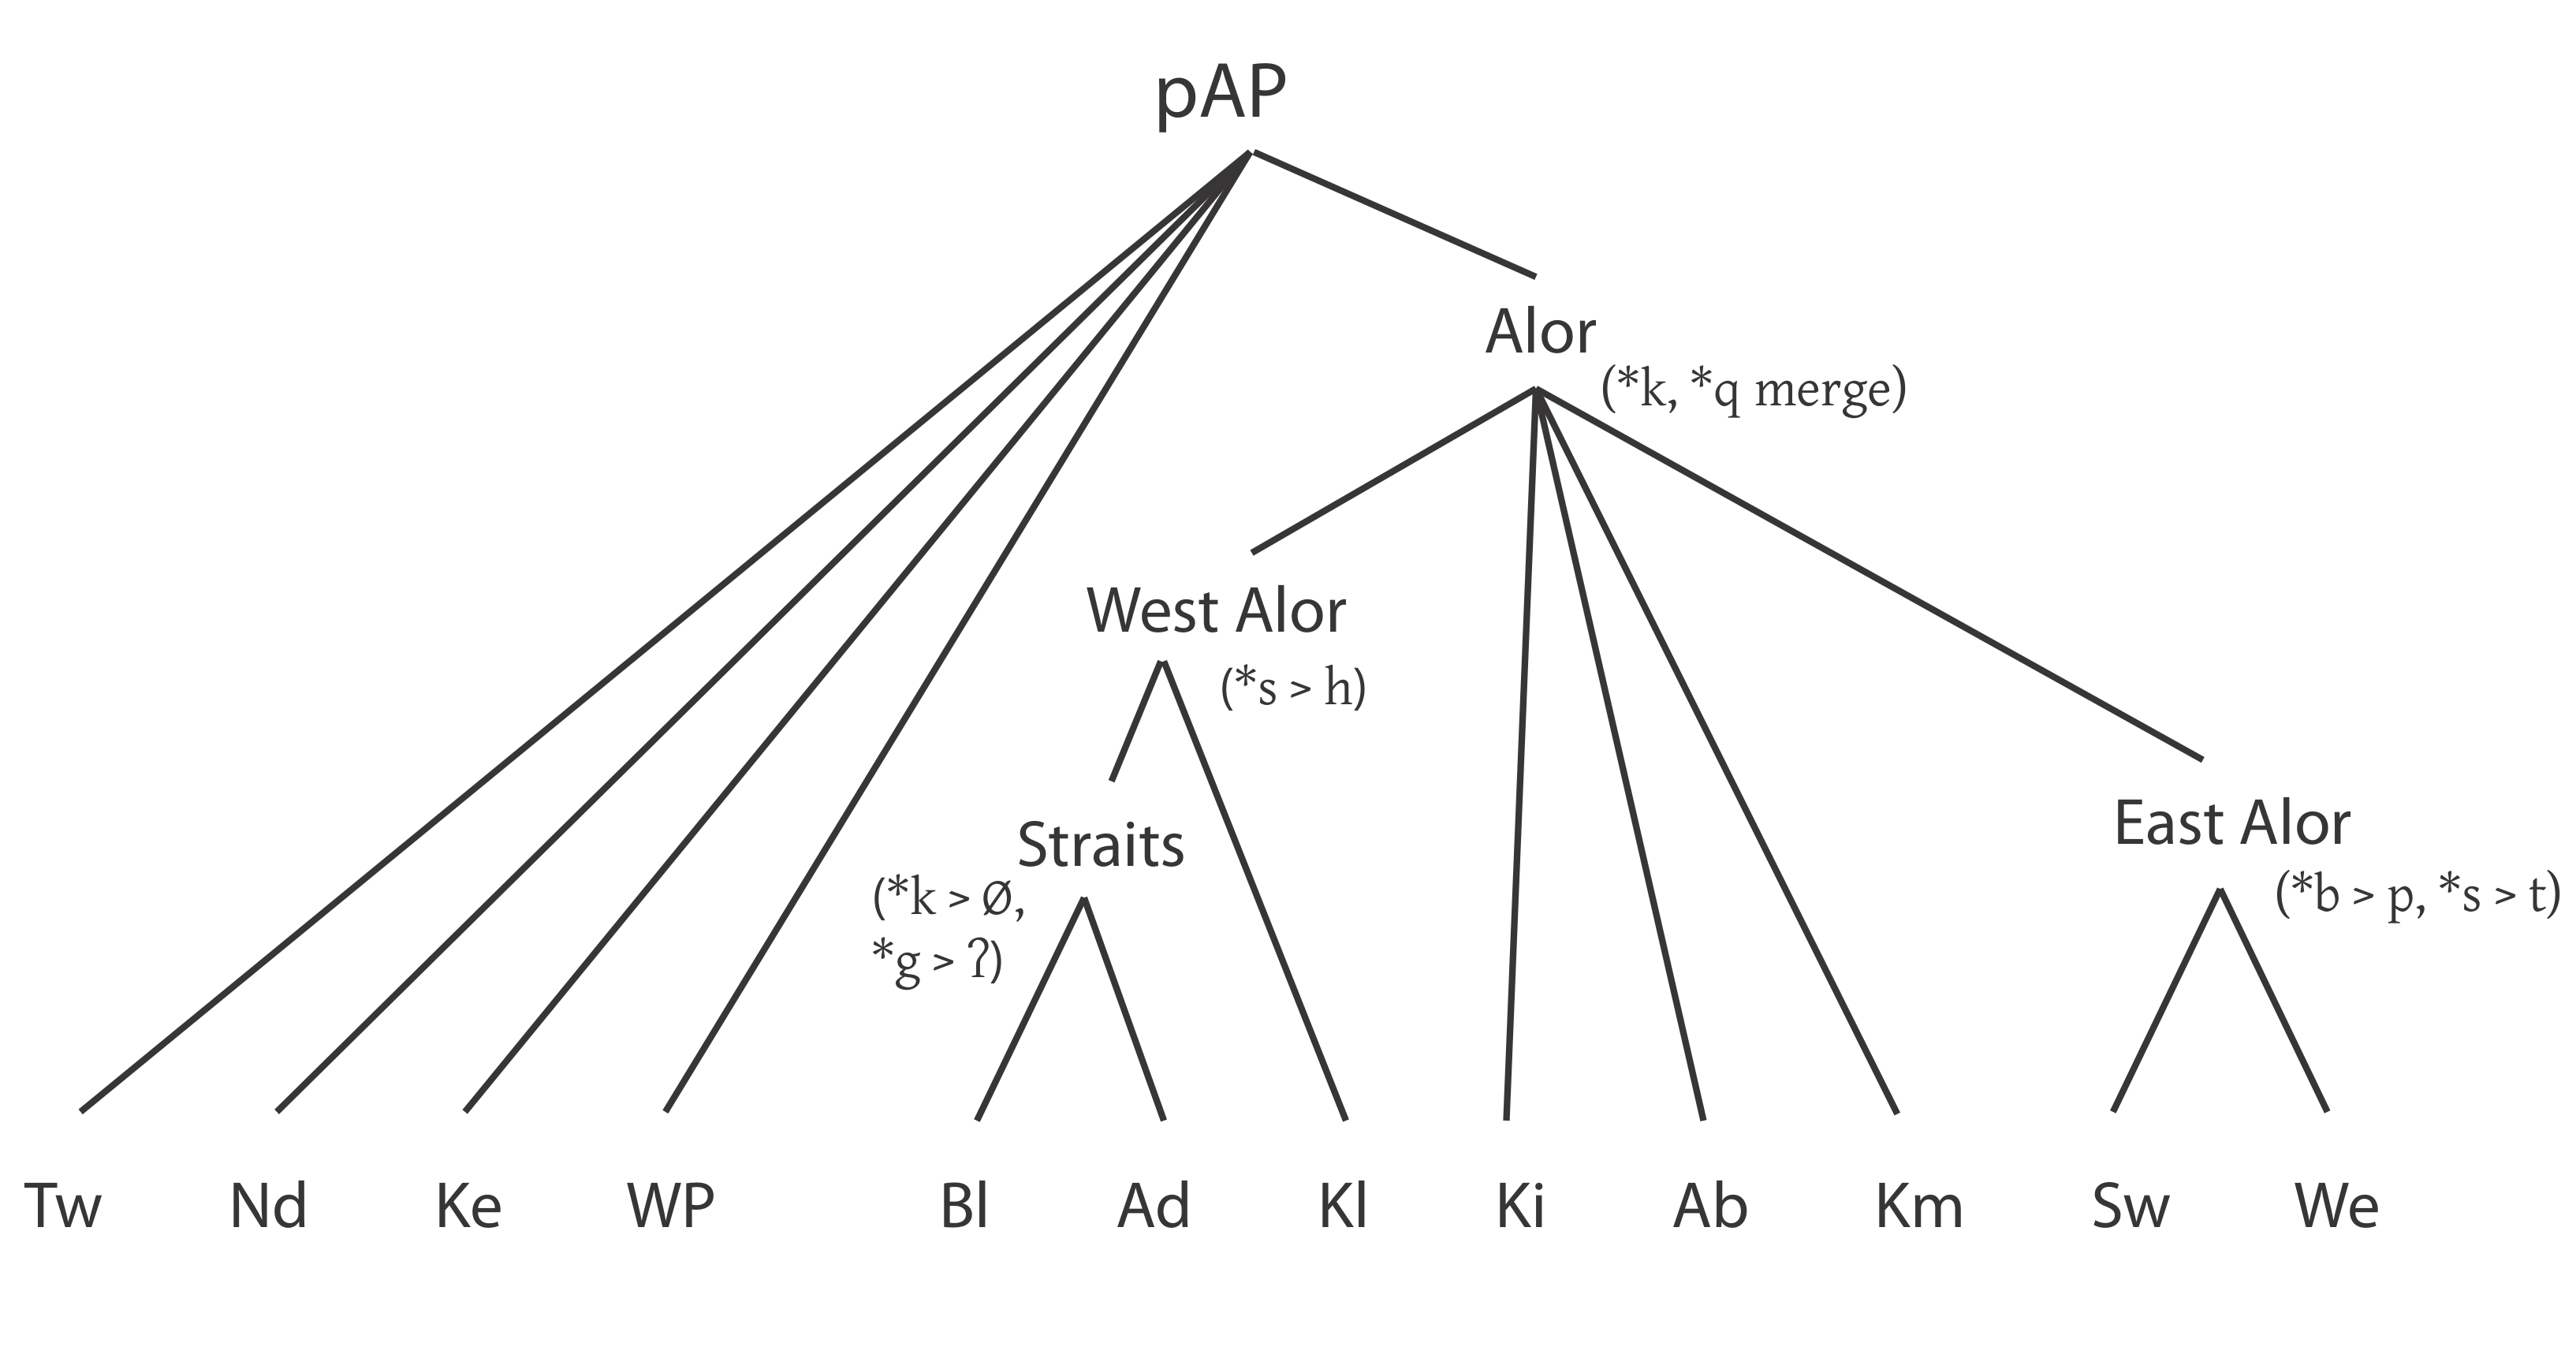
\includegraphics[width=\textwidth]{figures/holton_ch2_fig1.png}
\caption{Subgrouping of Alor-Pantar based on shared phonological innovations\ist{innovation}}
\label{fig:2:1}
\end{figure}

The tree based on shared phonological innovations\is{innovation} (Figure \ref{fig:2:1}) differs in several ways from previous classifications based on lexicostatistics. In particular, while the eastern languages Sawila and Wersing form a subgroup, they do not constitute primary branches of pAP\il{proto-Alor-Pantar}, as has been suggested in several previous classifications (cf. \citealt{Wurm1982}; \citealt{Lewis2009}). This tree has obvious geographic correlates, as shown in Figure \ref{fig:2:2} below. 

\begin{figure}[p]
\includegraphics[width=\textwidth]{figures/holton_ch2_fig2.pdf}
\caption{Distribution of subgroups defined based on shared phonological innovations\ist{innovation}}
\label{fig:2:2}
\end{figure}

The Alor subgroup defined by the merger of pAP velar and uvular stops includes all of the languages of Alor island and the intervening Pantar Straits. The languages of Pantar, with the exception of Blagar\il{Blagar} which is spoken on both Pantar and in the Straits, do not subgroup together. Within the Alor group are found two primary subgroups: East Alor at the eastern tip of the island, and West Alor comprising the western tip, the Bird's Head in the Northwest, and the Straits.

\subsection{ Subgrouping based on lexical characters}
A second approach to subgrouping delineates subgroups according to shared cognates. For each lexical correspondence set in our data we partitioned the languages into discrete cognate classes. As with the phonological innovations\is{innovation} discussed above, the lexical correspondence sets in our data do not all pick out the same subgroups. That is, the cognate sets delineated by some lexical items overlap with those delineated by other lexical items. These overlapping groupings can be visualized in a split graph which represents the distance between the characters in terms of numbers of splits (Figure \ref{fig:2:split_graph}). Details specific to our application of the method are laid out in \citet{RobinsonEtAl2012internal}.

\begin{figure}
\includegraphics[width=\textwidth]{figures/Ch2HoltonRobinsonAPhistoryMKprooftmp-img3.jpg}
\caption{Split graph of lexical character coded into cognate classes, generated using NeighborNet algorithm  \citep{HusonEtAl2006}. pAP node omitted for clarity.}
\label{fig:2:split_graph}
\end{figure}

Three primary regions can be identified in the graph, each separated by significant reticulation at the center of the graph. An East Alor region groups Kamang\il{Kamang}, Wersing\il{Wersing}, and Sawila\il{Sawila}; a Central Alor region groups Kui\il{Kui}, Klon\il{Klon}, and Adang\il{Adang}; and a Pantar region groups Kaera\il{Kaera}, Nedebang\il{Nedebang}, Teiwa\il{Teiwa}, and to a lesser extent Western Pantar\il{Western Pantar}. The high degree of reticulation within this latter group indicates a strong conflicting signal within this region. That is, of these three regions, the Pantar group is particularly non-tree-like, suggesting a pattern of wave-like innovations\is{innovation} in this region. In other words, although we found no shared phonological innovations\is{innovation} to subgroup these languages together in a traditional tree based on the comparative method (Figure \ref{fig:2:1}), these languages have borrowed a great deal from one another. 

A greater degree of reticulation in the graph represents a less tree-like signal in the data. The degree of tree-like signal can be quantified using the delta score metric \citep{WichmannEtAl2011,HollandEtAl2002}. The average delta score for our dataset is a moderately high $\delta $~=~0.29, reflecting the fact that while some groupings do emerge in Figure 3, there is significant reticulation between those groups. The most tree-like values are found in the East Alor grouping of Kamang\il{Kamang}, Wersing\il{Wersing}, and Sawila\il{Sawila}. The Pantar group of Teiwa\il{Teiwa}, Kaera\il{Kaera}, and Nedebang\il{Nedebang} has delta scores similar to the mean for the entire dataset; however, the value for Western Pantar\il{Western Pantar} is significantly higher, suggesting that similarities between Western Pantar and the remainder of the Pantar languages may be due more to borrowing\is{borrowing} than to shared descent. An unexpected result in the graph in Figure \ref{fig:2:split_graph} is the position of Blagar\il{Blagar} as a relative isolate within the family. In contrast to the subgrouping based on the comparative method, Blagar 
groups not with Adang and Klon but rather with the Pantar languages---and then only weakly so. 

A second method of subgrouping based on lexical characters uses Bayesian statistical techniques to search for trees which are most compatible with the cognate classes coded in our data.\footnote{ We employ a Markov Chain Monte Carlo (MCMC) method to search through the probability space of all possible trees, using a relaxed Dollo model. Details of this implementation can be found in \citet{RobinsonEtAl2012internal}, which compares the results of  several different models, using both MrBayes 3.2.1  \citep{RonquistEtAl2003} and BEAST 1.7.2 \citep{DrummondEtAl2012}, running each model for at least 10 million iterations with a sample rate of 1000 and a burn-in of 25 percent. Each model converged after approximately 1.5 million iterations, and the best performing model (i.e., that with the highest likelihood) was found to be the relaxed Dollo model implemented in BEAST. This model has been argued to be particularly appropriate to linguistic data, since it assumes that 
innovations\ist{innovation} may arise only once but may be lost multiple times independently \citep{Pagel2009}. } The results are summarized in Figure \ref{fig:2:bayes_mcc} as a maximum clade credibility tree. The clade credibility values listed below each node indicate the percentage of sampled trees which are compatible with that node. These values are for the most part either at or near one hundred percent (1.00), indicating that this consensus tree is compatible with almost all of the trees sampled in the analysis. Lower figures appear at exactly those nodes already shown to be problematic via the other subgrouping methods, namely Western Pantar\il{Western Pantar}, Abui\il{Abui}, and Kamang\il{Kamang}. 

\begin{figure}
%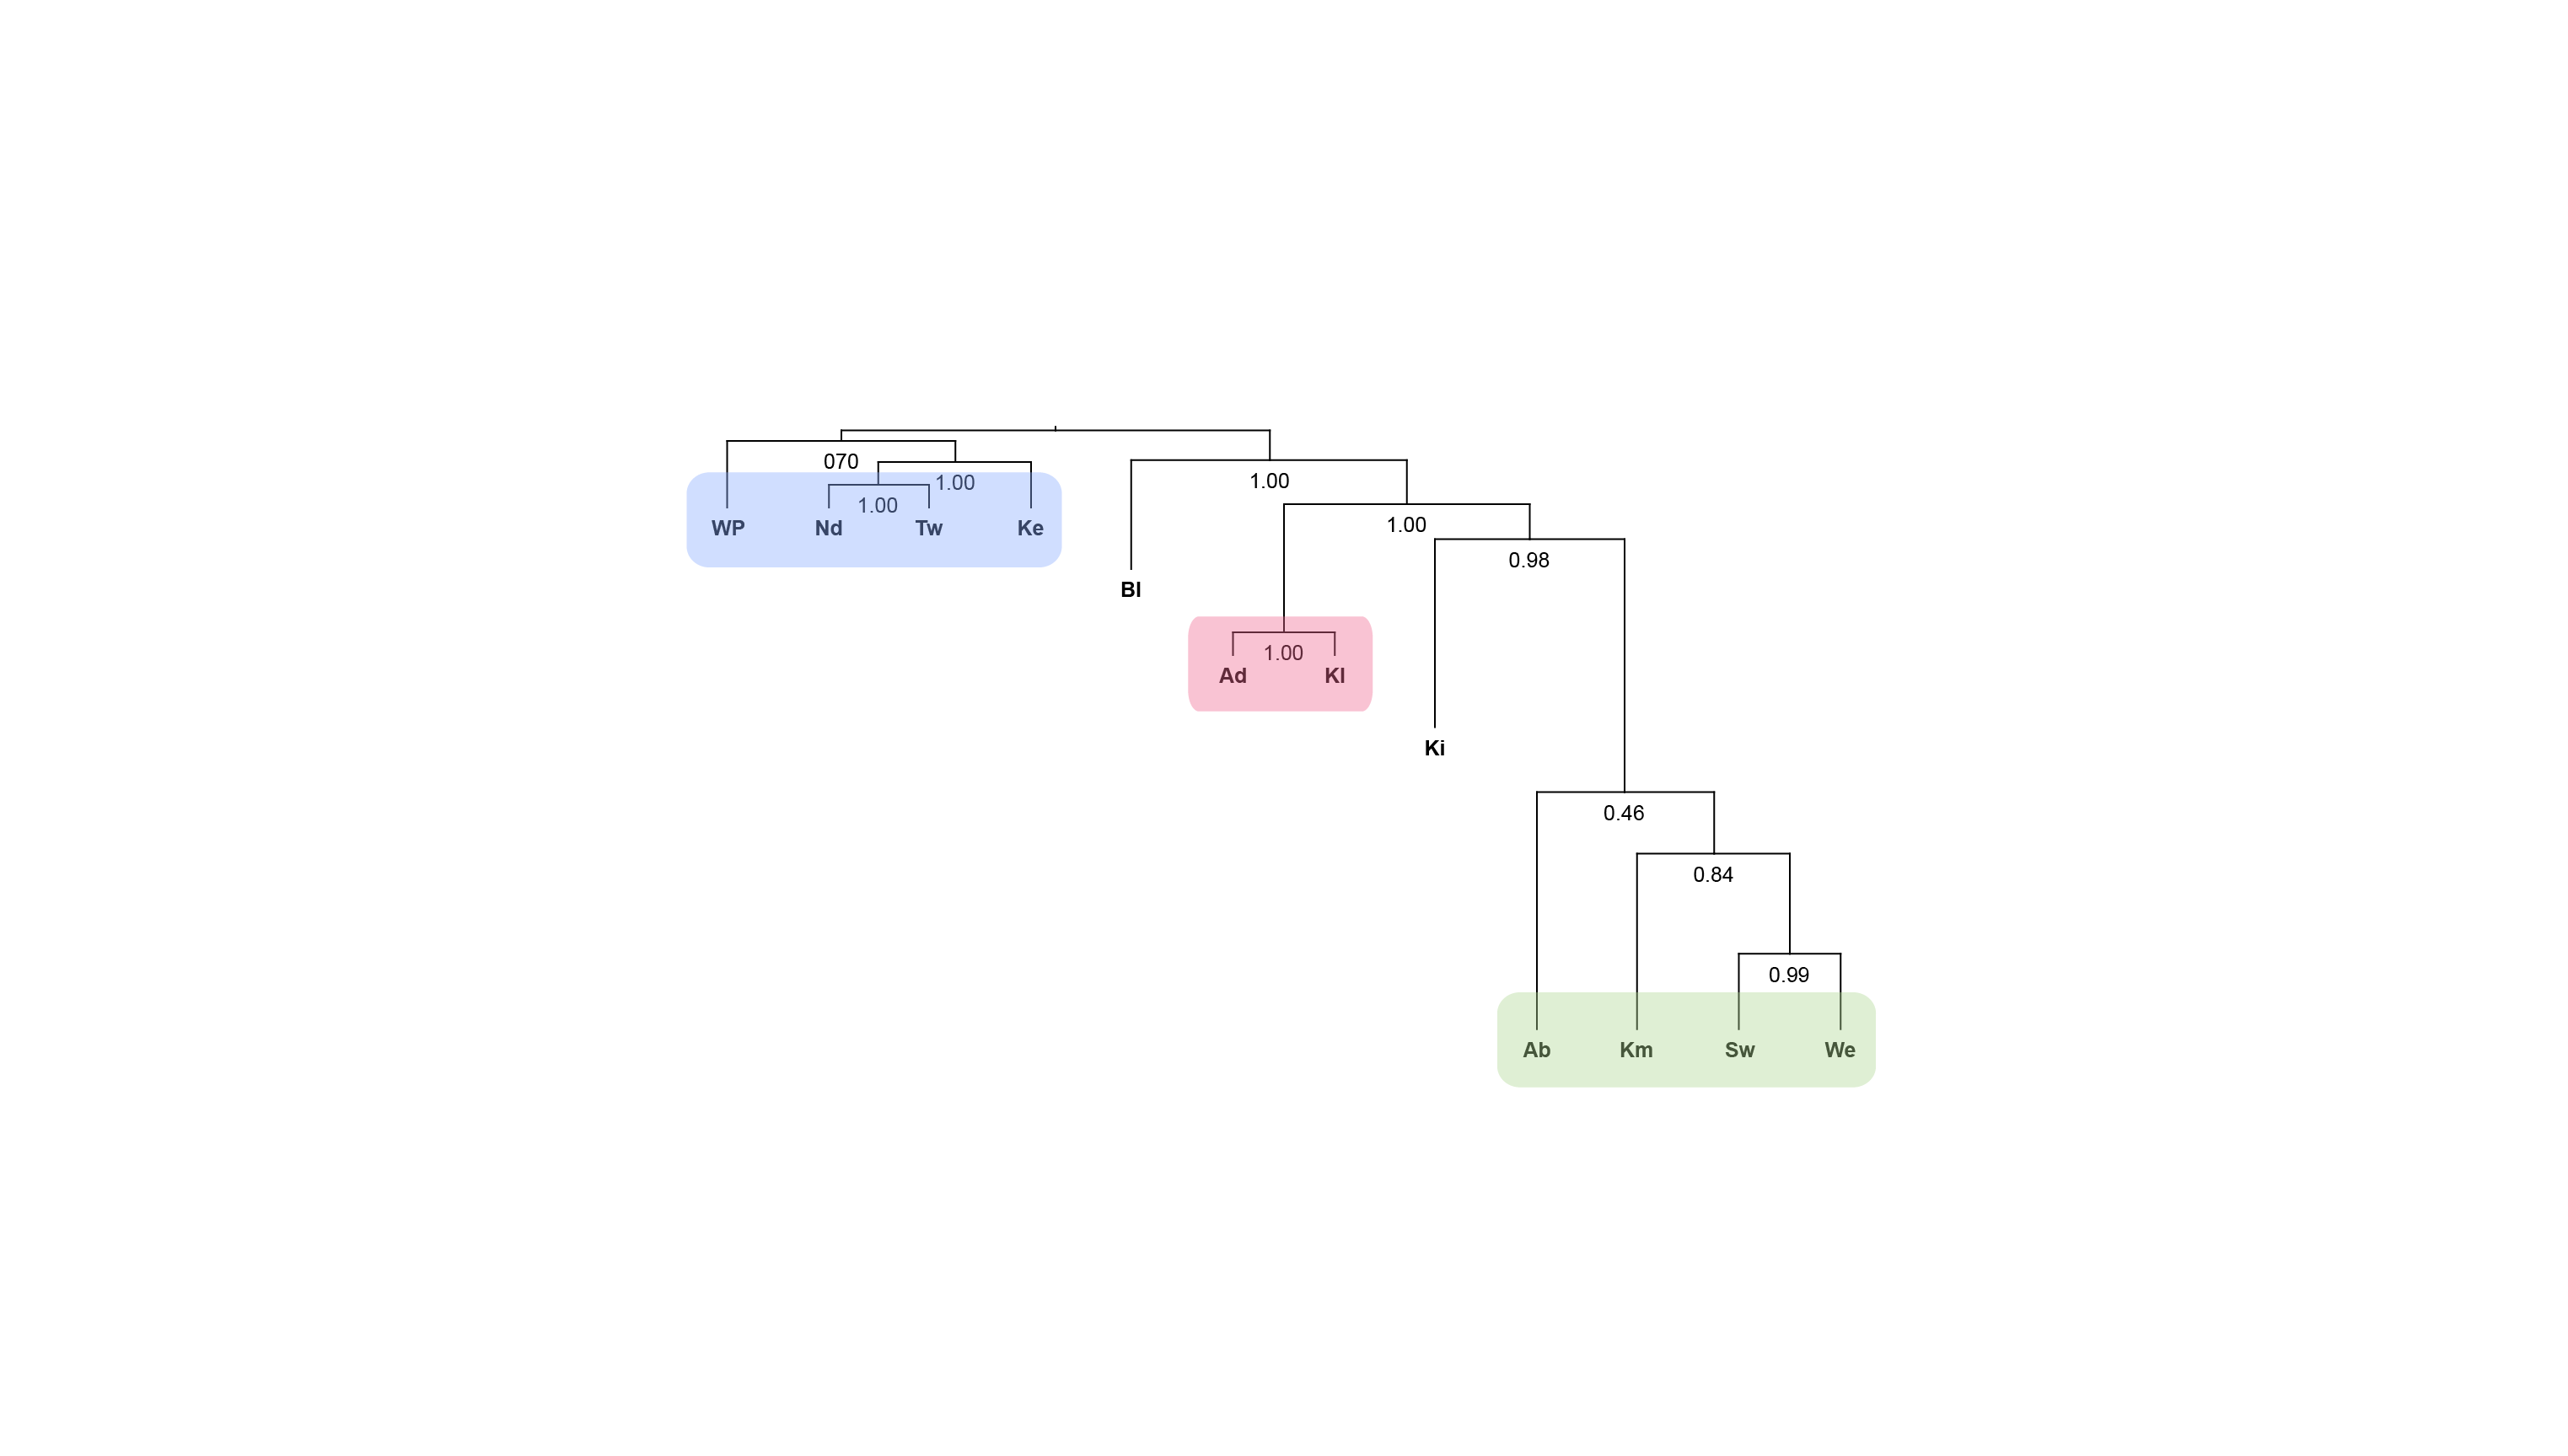
\includegraphics[width=\textwidth]{Ch2HoltonRobinsonAPhistoryMKprooftmp-img4.png}
\includegraphics[width=\textwidth]{figures/holton_ch2_fig4.pdf}
\caption{Bayesian MCMC maximum clade credibility tree for lexical data (relaxed Dollo model), with clade credibility values indicated. pAP\ilt{proto-Alor-Pantar} node omitted}
\label{fig:2:bayes_mcc}
\end{figure}

To a large extent the groupings in the Bayesian tree are compatible with those in the split graph. First, Sawila\il{Sawila} (Sw) and Wersing\il{Wersing} (We) are shown to be closely related, a grouping which was also present in the classification based on the comparative method (Figure \ref{fig:2:1}). Second, there is a Pantar grouping of Kaera\il{Kaera} (Ke), Teiwa\il{Teiwa} (Tw), Nedebang\il{Nedebang} (Nd), and Western Pantar\il{Western Pantar} (WP). Third, the position of Blagar\il{Blagar} (Bl) at the highest node coordinate to the Alor languages is consistent with its position in the split graph, though, as noted above, this differs significantly from its position in the tree based on the traditional application of the comparative method (Figure \ref{fig:2:1}). On the other hand, there are also some incompatibilities between the Bayesian tree and the split graph. For example, in the tree based on lexical characters Adang\il{Adang} (Ad) and Klon\il{Klon} (Kl) are shown forming a group without Kui\il{Kui} (Ki), contra both the splits graph and the tree calculated using the comparative method. 

Though not immediately apparent based on visual inspection of the maximum clade credibility tree in Figure \ref{fig:2:bayes_mcc}, the subgrouping based on lexical characters is also largely compatible with that based on phonological innovations\is{innovation}. To demonstrate this we repeated the Bayesian analysis with the constraint that all sampled trees be compatible with the subgroups identified by the comparative method, keeping all other parameters constant.\footnote{ The authors thank Michael Dunn for suggesting this innovative approach. } We then applied a marginal likelihood analysis to the results of each model, which yielded a Bayes factor of 1.1726, only slightly favoring the constrained model over the unconstrained one.\footnote{ Marginal likelihood was estimated using Tracer 1.5 \citep{RambautEtAl2007}.} The model based on lexical characters independently identifies the same subgroups found using a completely different methodology 
based on phonological characters, providing additional support for the robustness of the model. This lends support for those subgroups identified in the model based on lexical characters which are not found in the subgrouping based on phonological innovations\is{innovation}. In particular, we have some evidence for the existence of an East Alor subgroup comprised of Abui\il{Abui} (Ab), Kamang\il{Kamang} (Km), Sawila\il{Sawila} (Sw) and Wersing\il{Wersing} (We), even though this subgroup is not identified in the tree based on phonological characters. 

\section{Discussion}\label{sect_discussion}
The examination of sound correspondences across the Papuan languages of Alor and Pantar robustly supports the identification and reconstruction of an Alor-Pantar family. Our comparative work also allows us to propose internal subgroups within Alor-Pantar, but the overall linguistic picture is extremely complex, defying a model based solely on inheritance. Widespread multilingualism is the norm in the region, and borrowings\is{borrowing} from neighboring languages---such as Western Pantar\il{Western Pantar} \textit{bagis }`whine' from Deing\il{Deing} \textit{bagis} `cry'---are extremely common.\footnote{ Geographically, Deing lies between Western Pantar and Teiwa\ilt{Teiwa}. It appears to be closely related to Teiwa. } Additionally, genetic studies indicate that East Nusantara, and the Alor-Pantar region in particular, is a melting pot with a long history of admixture \citep{MonaEtAl2009}, and it may well be that an analogous situation holds for languages, reflecting extensive borrowing\is{borrowing} and metatypy\is{metatypy}. Thus it is not surprising that 
different methods reveal different trees for the family. 

The family tree based on phonological innovations\is{innovation} identified by the comparative method (Figure \ref{fig:2:1}) shows the highest level of diversity on Pantar, suggesting the languages originated in Pantar, spreading east. The tree based on the lexical characters (Figure \ref{fig:2:split_graph}) suggests that the languages of Alor originated in the Pantar Strait (around the area where Blagar is spoken today) with subsequent migration eastward. These two trees reveal different aspects of the prehistory of the AP languages. Phonological innovations\is{innovation} show the greatest degree of diversity on Pantar, suggesting a long history of settlement there. Lexical innovations\is{innovation} are compatible with an original settlement in the Pantar Strait. We propose that the original settlement was indeed in the area of the Pantar Strait with a very early split towards Pantar. That early settlement of Pantar led to the diversity we see there in terms of phonological innovations\is{innovation}. The lexical innovations\is{innovation} show less diversity on Pantar due to subsequent diffusion (as indicated by 
the significant reticulation for the languages of Pantar in Figure \ref{fig:2:split_graph}). As languages spread eastward from the Pantar Strait into Alor, new lexical innovations\is{innovation} were restricted to smaller and smaller subgroups in the east, leading to the embedded structure in the tree based on lexical characters (Figure \ref{fig:2:bayes_mcc}). However, the Pantar Strait languages (particularly Blagar\il{Blagar} and Adang\il{Adang}) constitute a more recent linguistic area across which phonological innovations\is{innovation} have been shared, leading to their close subgrouping in the tree based on phonological innovations\is{innovation} (Figure \ref{fig:2:1}).  

While this picture is fairly complex in terms of layers of history, it is not unexpected in a region of significant warfare and shifting alliances overlaid by several periods of contact from different outside groups (first the ancestors of today's Muslim speakers of Alorese\il{Alorese}, then the Dutch, and now Indonesian\il{Indonesian}). A more complete picture of the prehistory of the region must await evidence from other disciplines, particularly archaeology and genetics. 

\section*{Appendix}

\subsection*{Cognate sets}

Here we list 129 cognate sets reflecting regular sound correspondences. There are only 127 distinct meanings, as two of the meanings, `dog' and `walk', are found in more than one cognate set; these are indicated with subscripts following the gloss. In the table the correspondence sets are listed alphabetically by English gloss. Languages are arranged in order roughly from west to east with the western-most languages on the left and the eastern-most languages on the right. Correspondence sets may include irregular forms when they serve to demonstrate the correspondence under discussion. In these cases the irregular forms are denoted with a preceding double dagger ({\ddag}). We reconstruct pAP\il{proto-Alor-Pantar} forms only when we have broad geographic support in minimally one language of Pantar (Teiwa\il{Teiwa}, Nedebang\il{Nedebang}, Kaera\il{Kaera}, Western Pantar\il{Western Pantar}), one language of West Alor and the Pantar Strait (Blagar\il{Blagar}, Adang\il{Adang}, 
Klon\il{Klon}, Kui\il{Kui}), and one language of East Alor (Abui\il{Abui}, Kamang\il{Kamang}, Sawila\il{Sawila}, Wersing\il{Wersing}). Of these 129 correspondences, 117 reconstruct to the level of pAP\il{proto-Alor-Pantar}.


\begin{sidewaystable}
\footnotesize
\setlength{\tabcolsep}{1pt}
\begin{tabularx}{\textwidth}{lc>{\it}c>{\it}c>{\it}c>{\it}c>{\it}c>{\it}c>{\it}c>{\it}c>{\it}c>{\it}c>{\it}c>{\it}c}
\lsptoprule
Gloss & \rm pAP\ilt{proto-Alor-Pantar} & \rm Tw\ilt{Teiwa} & \rm Nd\ilt{Nedebang} & \rm Ke\ilt{Kaera} & \rm WP\ilt{Western Pantar} & \rm Bl\ilt{Blagar} & \rm Ad\ilt{Adang} & \rm Kl\ilt{Klon} & \rm Ki\ilt{Kui} & \rm Ab\ilt{Abui} & \rm Km\ilt{Kamang} & \rm Sw\ilt{Sawila} & \rm We\ilt{Wersing}\\
\midrule 
{`axe'{\tablenote}} & & & & & {bali{\ng}} & & {bali{\ng}} & & & {fali{\ng}} & {pali{\ng}} & &  \\
`bad, broken' & *jasi & jas & jet{\textesh}i & jas- & jasa & d{\textyogh}asi & sah & ja{\textlengthmark}h &  &  &  & ja{\textlengthmark}ti & \\
`bamboo' & *mari &  &  &  & mali & mari & mai & (du)mar &  & ma{\textlengthmark}i & ma{\textlengthmark}i &  & \\
`banana' & *mogol & mu{\pharfric}ui & {\ddag}maj & mogoi & mag{\textlengthmark}i & {\ddag}m{\textopeno}l & m{\textopeno}{\textglotstop}{\textopeno}i & m{\textschwa}gol &  &  & mo{\textlengthmark}i &  & mulul\\
`bark' (v.) & *lVu &  &  &  & lau & {\ddag}orow & lou &  &  & loi &  & lu & aloi\\
`bat' & *madel & m{\textschwa}di & {\ddag}mara & {\ddag}merei & mad{\textlengthmark}e & d{\textepsilon}m{\textepsilon}l{\tablenote} & {\ddag}madiru{\ng} & m{\textschwa}d{\textepsilon}l & madel & marel & matei & {\ddag}madi{\textlengthmark}(ku) & {\ddag}mudu(k)\\
`bathe' & *weli & wei &  & wei &  & v{\textepsilon}la & foil & w{\textepsilon}{\textlengthmark}l & weli &  -wel &  -wei & wile &  -weli\\
`bedbug' & *temek &  &  & temek &  & t{\textepsilon}m{\textepsilon} & {\ddag}tame{\textglotstop} & tamek &  & tameki &  &  & mekit{\tablenote}\\
`betel~nut' & *bui  & bui  & buja  & bui  & bu  & bu  & bu  & bui  & bui  & fu  & & pu  & pui \\
`betel vine' & *mait & met & mata & mat & meta & mat & met{\textesh} & meh & mesin & me{\textlengthmark}ti{\ng} & maisi & ma{\textlengthmark}si & mas\\
`bird' & *(a)dVl & dai & {\ddag}daja &  &  & {\ddag}du{\ng} &  &  & adol & ruwol{\tablenote} & atoi & adala & adol\\
`bite' & *asi & si & t{\textesh}ia & si{\textlengthmark} & sia &  &  -eh & {\textepsilon}h &  -es &  &  -eh &  & \\
`black' & *aqana & qa{\textglotstop}an & qana & xan & {\ddag}ana & ka{\textglotstop}ana & (l)a{\textglotstop}an & akan & akana & akan &  & akana & ake{\ng}\\
`blood' & *wai & wai & we & wei & wai & v{\textepsilon} & foi & we{\textglotstop} & we & wea & we{\textlengthmark} & wi{\textlengthmark} & wei\\
`body~hair' & *mudi & mud & mudi &   -mudu &  &  -mudi &  & amudi &  & amur &  & madi & mudi\\
`bone' &  & kir & kili & kiri &  & kira &  &  &  &  &  &  & \\
`breast' & *hami &  -{\pharfric}am & ami &  &  -ha{\ng} &  &  &  &  &  & ami &  -a{\textlengthmark}mi & ami\\
`burn' & *ede & de{\textglotstop} &  & de &  & {\textglotstop}{\textepsilon}de &  &  &  & {\ddag}diei &  &  & \\
`child' & *uaqal &  -oqai & uaqa &  -uax & wak{\textlengthmark}e &  -oal & {\textglotstop}ai & {\ddag}ul & {\ddag}ol &  &  &  & {\ddag}ol\\
`climb' & *mid & mir &  &  & mid{\textlengthmark}a{\ng} &  & mid & mid &  &  &  & mada & \\
`close' (v.) & *-tiari(n) &  &  & teri{\ng} & {\ddag}tiari{\ng} & t{\textepsilon}ri{\ng} & t{\textepsilon}l & (u)t{\textepsilon}r & (u)t{\textepsilon}ri &  &  &  -ti{\textlengthmark}ra & (le)ter\\
`coconut' & *wata & wat & wata & wat & wata & v{\textepsilon}t & fa & {\ddag}ata & {\ddag}bat & wata & wate & wata & wata\\
`come' & *mai{\tablenote} & ma & ma & ma & ma & ma & ma & ma & mai & m{\textepsilon} & me{\textlengthmark} & me & amai\\
`crocodile' & *bagai  & {ba{\pharfric}a{\textlengthmark}i} & & bagai  & {{\ddag}bagai} & & {ba{\textglotstop}ai} & {b{\textschwa}gai} & {{\ddag}buai} & fahai  & {pie{\textlengthmark}} & &  \\
`crouch' & *luk(V) &  &  &  & luk{\textlengthmark}i{\ng} &  &  &  & luk  & lu{\textlengthmark}k{\tablenote} & luk{\tablenote} &  & luku(k)\\
`die' & *min(a) & min & mina & nimin & {\ddag}hin{\textlengthmark}a & mina & min &  & min & mo{\ng} &  &  & \\
`dog\textsubscript{1}' & *jibar{\tablenote} & ji{\textprimstress}var & {\ddag}bar & i{\textprimstress}bar & ja{\textprimstress}b{\textlengthmark}e & d{\textyogh}a{\textprimstress}bar & bel &  &  &  &  &  & \\
\lspbottomrule
\end{tabularx}
\end{sidewaystable}

\begin{sidewaystable}
\footnotesize
\setlength{\tabcolsep}{1pt}
\begin{tabularx}{\textwidth}{lc>{\it}c>{\it}c>{\it}c>{\it}c>{\it}c>{\it}c>{\it}c>{\it}c>{\it}c>{\it}c>{\it}c>{\it}c}
\lsptoprule
Gloss & \rm pAP\ilt{proto-Alor-Pantar} & \rm Tw\ilt{Teiwa} & \rm Nd\ilt{Nedebang} & \rm Ke\ilt{Kaera} & \rm WP\ilt{Western Pantar} & \rm Bl\ilt{Blagar} & \rm Ad\ilt{Adang} & \rm Kl\ilt{Klon} & \rm Ki\ilt{Kui} & \rm Ab\ilt{Abui} & \rm Km\ilt{Kamang} & \rm Sw\ilt{Sawila} & \rm We\ilt{Wersing}\\
\midrule
`dog\textsubscript{2}' &  &  &  &  &  &  &  & ku{\textlengthmark}r & kur & ka{\textlengthmark}i & kui &  & \\
`dream' & *hipar &  &  & ipar & hip{\textlengthmark}e & ipar & apai & eper &  & piei &  -foi &  & \\
`dry in sun' & *por &  &  & pori{\ng} & {\ddag}puari{\ng} & pori{\ng} & poil & upu{\textlengthmark}r &  &  &  & po{\textlengthmark}por{\tablenote} & \\
`dry' &  &  &  &  &  & {\ddag}ta{\textglotstop}ata & ta{\textglotstop}at & t{\textschwa}kat & takata & takat &  &  & \\
`ear' & *uari & uar & ow & uar & uwe & v{\textepsilon}ri &  -fel & wer & {\ddag}wel & wei & wai &  -wari & weri\\
`eat/drink'{\tablenote} & *nai & na & ina & na & na & na & na & na{\textlengthmark}{\textglotstop} & nai & ne{\textlengthmark} & ne & ne{\textlengthmark} & nai\\
`empty' & *hasak & hasak &  & isik & hak{\textlengthmark}as{\tablenote} &  &  &  &  & taka & saka &  & \\
`excrement' & *has & {\pharfric}as &  &  & has & {\ddag}a{\textlengthmark}s & ah & ihi & es & {\ddag}asi & asi & atu & atu\\
`expel' & *tiara &  -tiar &  -tiala & ter &  &  -t{\textepsilon}ri & (at{\textepsilon})t{\textepsilon}l &  &  &  &  & ti{\textlengthmark}ra &  -(pan)ter\\
`far' & *lete{\tablenote} &  &  &  &  &  & l{\textepsilon}t & l{\textepsilon}t &  &  & letei &  & \\
`fat'  & *tama & tama{\textglotstop} &  & tama &  & tama & tama(r) & t{\textschwa}ma(d) & tama & tama(da) &  &  & \\
`father' & *-mam &  &  &  -mam &  &  -ma{\ng} &  -ma{\ng} &  -man & {\ddag}-ma & ma{\textlengthmark}ma &  &  & \\
`fingernail' & *kusin &  & kut{\textesh}i{\ng} & kusi{\ng} & {\ddag}kusi & {\ddag}kusil & {\textglotstop}uhuin & {\ddag}kuh & kusin & {\ddag}kus{\textsci}{\ng} & kuisi{\ng} &  & \\
`fire' & *hada & {\pharfric}ar & ar & ad & had{\textlengthmark}i{\tablenote} & {\textglotstop}ad & {\ddag}a & ada{\textglotstop} & ar & ara & ati & ada & ada\\
`fish' & *habi & {\pharfric}a{\textphi} & a{\textlengthmark}fi & ab & hap & a{\textlengthmark}b & ab & ibi{\textglotstop} & eb & afu & api & api & api\\
`five' & *jiwesin & jusan & {\ddag}jisin & isim & jasi{\ng} & {\ddag}isi{\ng} & ifihi{\ng} & {\textepsilon}w{\textepsilon}h & jesan & jeti{\ng} & iwesi{\ng} & jo{\textlengthmark}ti{\ng} & weti{\ng}\\
`flea' & *kVt & {\ddag}{\pharfric}at &  &  & kati &  & {\ddag}{\textglotstop}ut &  & kot &  &  &  & toko{\textglotstop}{\tablenote}\\
`fly' (v.) & *jira(n) & jir-an & jila & ir & hil{\textlengthmark}a{\ng} &  &  &  &  &  &  & iri{\ng} & ire\\
`fruit' & *is(i){\tablenote} & jis & it{\textesh}i & isi & {\ddag}his{\textlengthmark}a & ({\textglotstop})ihi &  & ih &  &  & ih & {\ddag}-si & {\ddag}-is{\tablenote}\\
`garden' &  & ma{\pharfric}ar & maxara &  & mag{\textlengthmark}ar &  & ma{\textglotstop}ad &  &  &  &  &  & \\
`give' & *-enV &  -an &  -ena &  -e{\ng} &  -nia &  -{\textepsilon}na{\ng} &  -{\textepsilon}n &  -en &  -ana &  &  -n &  &  -eni(r)\\
`good' &  &  &  &  &  &  & n{\textopeno}{\textglotstop} & nok & noka &  &  &  & \\
`guard' & *bukan & {\ddag}bo{\pharfric}on &  & buka{\ng} & bauka{\ng} &  &  & bu{\textlengthmark}k &  &  &  -pukan &  & \\
`hand/arm' & *-tan &  -tan &  -ta{\ng} & ta{\ng} & t{\textlengthmark}a{\ng} & ta{\ng} & ta{\ng} & tan & tan & ta{\ng} & ta{\ng} & ta{\ng} & te{\ng}\\

\lspbottomrule
\end{tabularx}
\end{sidewaystable}

\begin{sidewaystable}
\footnotesize
\setlength{\tabcolsep}{1pt}
\begin{tabularx}{\textwidth}{lc>{\it}c>{\it}c>{\it}c>{\it}c>{\it}c>{\it}c>{\it}c>{\it}c>{\it}c>{\it}c>{\it}c>{\it}c}
\lsptoprule
Gloss & \rm pAP\ilt{proto-Alor-Pantar} & \rm Tw\ilt{Teiwa} & \rm Nd\ilt{Nedebang} & \rm Ke\ilt{Kaera} & \rm WP\ilt{Western Pantar} & \rm Bl\ilt{Blagar} & \rm Ad\ilt{Adang} & \rm Kl\ilt{Klon} & \rm Ki\ilt{Kui} & \rm Ab\ilt{Abui} & \rm Km\ilt{Kamang} & \rm Sw\ilt{Sawila} & \rm We\ilt{Wersing}\\
\midrule 

`hear' & *magi{\tablenote} &  &  &  &  & m{\textepsilon}{\textglotstop}{\textepsilon} & ma{\textglotstop}eh & m{\textschwa}gih & magi & mahi & mai & maji{\textlengthmark}{\ng} & \\
`hearth' &  & tuta({\pharfric}) & tutu- & tutu(k) & tut{\textlengthmark}u & tutu &  &  &  &  &  &  & \\
`hold'{\tablenote} & *p\{i,u\}nV & pin & pini & pin & pin{\textlengthmark}i & pina & puin & puin & puna & pun & fun & puni{\tablenote} & poi{\ng}{\tablenote}\\
`horn' & *muk &  &  & muk &  & mu & mu & muk & muk & muk & {\ddag}mu{\textlengthmark} &  & \\
`(be) in/on' & *mi & me{\textglotstop} &  & mi & me & mi & mi & mi & mi & mi & mi & ma & \\
`itchy' &  & qa{\textlengthmark}q & qaqa & xaxaw & kaka & kaka & {\ddag}kak & ka{\textlengthmark}k &  &  &  &  & \\
`knee' & *uku & ku{\textlengthmark}{\textglotstop} & uku & uku & uk{\textlengthmark}a({\ng}) & (k)uku &  &  -uk &  -uk &  &  & (ta{\textlengthmark}sur)uku & (seseb)uk\\
`laugh' & *jari & {\ddag}ja{\pharfric}ar & {\ddag}gela & {\ddag}agar & jali &  & asal & {\ddag}{\textglotstop}{\textschwa}gar & jeri &  & {\ddag}je{\textlengthmark}i & jara & jer\\
`leg' & *-bat{\tablenote} &  -{\textphi}at &  &  -bat &  -uta &  &  -({\textepsilon}{\textglotstop})fa &  &  &  &  &  & \\
`lime' & *hawar & {\pharfric}or & wa & awar & hauwe & avar & {\textglotstop}afai & {\textepsilon}w{\textepsilon}r & o{\textlengthmark}r & awai & awoi &  & or\\
`lizard' &  & takok & taka(ra:b) & tek & tak{\textlengthmark}e & t{\textepsilon}k{\textepsilon} & {\ddag}t{\textepsilon}k{\textopeno} & takek & takok & tekok & {\ddag}tak{\textlengthmark}e{\textlengthmark} & tako & \\
`maize' & & batar  & {ba{\textlengthmark}ta} & batar  & {bat{\textlengthmark}e} & batar  & {bat{\textepsilon}} & bat  & batar  & fat  & patei  & patara  & peter \\
`mat' & *bis & bis & {\ddag}bi{\textlengthmark} & bis & bis & bihi & buh &  & bus & fut &  & {\ddag}bu{\textlengthmark}si & {\ddag}biti{\textglotstop}\\
`moon' & *wur & wur & hula & ur &  & uru & ul & ur & ur &  & wui &  & ura(k)\\
`mosquito' & *kin & ki{\textglotstop}in & kim(balu) & ki{\ng} & ki{\tablenote} & kini & {\textglotstop}in & ikin & kin &  & ki{\ng}(ba) & ka(we:{\ng}) & ku(bu{\ng})\\
`mouth'{\tablenote} & *-wa &  -aw &  -wa &  -ua &  -wa(r) &  -va &  -(ar)fah &  &  &  -wa &  -wa{\textlengthmark} &  -wa &  -wa\\
`name' & *-en(i,u) &  &  -einu &  -en &  -in{\textlengthmark}u &  -{\textepsilon}n{\textepsilon} &  -ni &  -n{\textepsilon}{\textglotstop} &  -enei &  -ne &  -nei &  -ni & \\
`new' & *siba & {\ddag}sib & sava({\textglotstop}a) & sib & sab{\textlengthmark}a{\tablenote} & hiba & haba(r) & h{\textschwa}ba & saba & tif{\textscripta} & supa(ka) & tipea & t{\textschwa}pa\\
`nose' & *-mim &  &  &  -mim & {\ddag}-m{\textlengthmark}i &  -mi{\ng} &  -mi{\ng} &  -muin &  -min &  &  &  -mi{\ng}i &  -mui{\ng}\\
`one' & *nuk & nuk & nuku & nuk & anuku & nu & nu & nuk & nuku & nuku & nok &  & no\\
`pierce'{\tablenote} & *tapai & tap & tapa & tap & tap{\textlengthmark}a({\ng}) & tapa & tapa({\ng}) & tapa(n) & tapai & tapei & tafe &  & ta\\
`pig' & *baj  & bai  & bei  & bei  & bai  & {b{\textepsilon}} & boi  & {be{\textglotstop}} & bei~  & fe  & pe  & pi  & pei \\
`plant'~(v.) & *mudin & midan & mudi & mudu{\ng} & mid{\textlengthmark}i{\ng} & mudi{\ng} & mudi{\ng} & mdin & medi & murui & mit & madi{\ng} & m{\textschwa}di\\
`rat' & *dur & dur & dur & dur & di & duru & {\ddag}dur & dur & dur & rui & tui & daru & dur(ki)\\
`rattan' &  & liag &  & le{\textlengthmark}g &  & {\textglotstop}ilia & l{\textepsilon} &  & le &  &  &  & \\
`recline' & *tia & ti{\textlengthmark}{\textglotstop} & ta{\textglotstop}a & te & ti{\textglotstop}a{\ng} & tia &  & ta{\textlengthmark} & ta & ta{\textlengthmark} & ta{\textlengthmark}{\tablenote} &  -te & taj\\
`right' &  & jidan & jedi{\ng} &  & jad{\textlengthmark}i{\ng} &  &  &  &  &  &  &  & \\

\lspbottomrule
\end{tabularx}
\end{sidewaystable}

\begin{sidewaystable}
\footnotesize
\setlength{\tabcolsep}{1pt}
\begin{tabularx}{\textwidth}{lc>{\it}c>{\it}c>{\it}c>{\it}c>{\it}c>{\it}c>{\it}c>{\it}c>{\it}c>{\it}c>{\it}c>{\it}c}
\lsptoprule
Gloss & \rm pAP\ilt{proto-Alor-Pantar} & \rm Tw\ilt{Teiwa} & \rm Nd\ilt{Nedebang} & \rm Ke\ilt{Kaera} & \rm WP\ilt{Western Pantar} & \rm Bl\ilt{Blagar} & \rm Ad\ilt{Adang} & \rm Kl\ilt{Klon} & \rm Ki\ilt{Kui} & \rm Ab\ilt{Abui} & \rm Km\ilt{Kamang} & \rm Sw\ilt{Sawila} & \rm We\ilt{Wersing}\\
\midrule

`ripe' & *tena &  &  & ten &  & t{\textepsilon}na & t{\textepsilon}n & {\textepsilon}t{\textepsilon}n & tain &  & iten & iti{\textlengthmark}na & \\
`roof' & *wai & wai & waja &  & wai & vai & fa & wei & wai & wa{\textlengthmark}i & iwa{\textlengthmark}h{\tablenote} &  & \\
`rotten' & *mVn & mu{\textlengthmark}n &  -mini & mino &  & min(isa) & {\ddag}mul & muin &  &  -mun &  &  & \\
`saltwater' & *tam & {\ddag}ta{\textglotstop} & ta & tam & tawa & ta{\ng} & ta{\ng} & tan & tan & tama & tama & tama & tama{\textglotstop}\\
`scorpion' & *pVr & par &  & par & {\ddag}par & {\ddag}p{\textepsilon}l & pail & par & per & pe{\textlengthmark}i & {\ddag}fal &  & per(buk)\\
`search' &  &  & lafi & rap &  & rapi{\ng} & lap &  &  -rap &  &  &  & \\
`shark' & *sib(a,i)r{\tablenote} & si{\textphi}ar & sifi & sibar & sib:u & hibir & {\ddag}tab{\textepsilon}i &  & sobor &  &  &  & \\
`short' & *tukV & tuk & tuku & tuk & tuk:a & tuka({\ng}) & to{\textglotstop}a({\ng}) & tuk & tuk & tuku{\tablenote} & tuk{\tablenote} & tuku(da) & tuk\\
`sibling (older)' & *nan(a) &  &  -na{\ng} &  &  &  &  &  &  & na{\textlengthmark}na &  &  -na{\textlengthmark}na &  -na{\ng}\\
`sing' & *dar(a) & da{\textlengthmark}r & da{\textlengthmark}la{\tablenote} & da{\textlengthmark}ro{\tablenote} & dali & dar & dal &  & dar & jai{\tablenote} &  & dara & d{\textschwa}ra\\
`sit' & *mis & mis & misi & mis- & mis(i{\ng}) & mihi & mih & mih & misa & mit & {\ddag}nih & miti & amit\\
`six' & *talam & {\ddag}tia{\textlengthmark}m & {\ddag}tiama & {\ddag}tiam &  & tali{\ng} & tala{\ng} & t{\textschwa}lan & talama & tala{\textlengthmark}ma & ta{\textlengthmark}ma &  & \\
`sky' &  & bulan &  & bulu{\ng} &  & {\ddag}bura{\ng} &  &  &  &  &  &  & \\
`slippery' & *dul(a) &  &  & duj- & {\ddag}duba & dula & dul & du{\textlengthmark}l & dula & rula & tula(ka) & dalo{\textlengthmark}(ka) & dol(ok)\\
`smoke' & *bunaq & bu{\textlengthmark}n & bun & banax & bun{\textlengthmark}a & benaka & bano{\textglotstop} &  -bon & bonok &  & puna & punaka & punak\\
`spear' & *qaba(k) & {\ddag}qab & {\ddag}qaba & xabi & kab{\textlengthmark}i & {\textglotstop}aba & {\textglotstop}aba & k{\textschwa}bak & kabak & kafak & kapa &  & \\
`spit' & *purVn & puran & (mali)plum & pura{\ng} &  & puru{\ng} & pui & p{\textschwa}ruin & puri{\ng} & puina & (su)pui &  & \\
`stand' & *tas & tas & tasi & tas- &  & tahi & toh & (m{\textschwa})t{\textepsilon}h &  & (na)tet &  &  &  -tati\\
`star' & *jibV & ji{\textphi} & ifa(xoja) & {\ddag}ip(alaq) & hib{\textlengthmark}i & {\ddag}i{\textlengthmark}d & ib(i{\ng}) & {\textglotstop}ib & ib(ra) &  &  &  & \\
`stomach' & *-tok & {\ddag}-to{\textglotstop} & {\ddag}-to{\textglotstop}o &  -toki &  &  -tow &  -to{\textglotstop} &  &  &  &  -tok &  &  -toko\\
`stone' & *war & war & wala & war &  & var & f{\textopeno}i & w{\textopeno}r & wor & wi & woi & wara & wor\\
`sugarcane' & *hu{\textlengthmark}ba & {\ddag}hub{\tablenote} & u{\textlengthmark}fa & u{\textlengthmark}b & habua & ub & {\ddag}sob & aba & u{\textlengthmark}b &  &  &  & upa\\
`sun' & *wadi & war (get) & weri & {\ddag}wer & war{\tablenote} & v{\textepsilon}d & fed &  & {\ddag}ber & war & wati & wadi & widi\\
`tail' & *ora &  -or & ola &  -or &  &  -ora & ol &  -{\textopeno}r &  -or &  -wai & (w)ui & (w)o{\textlengthmark}ra & (w)ori\\
`tooth' & *uasin & usan & usi{\ng} & uasi{\ng} & wasi{\ng} & {\ddag}\textit{{}-}vei{\ng} & fihi{\ng} &  -weh &  -wes &  -weti &  -weh & {\ddag}-wa & {\ddag}wesi\\
`tens'{\tablenote} & *qar- & qa{\textlengthmark}r- & qa- & xar & ke- & {\textglotstop}ar- & {\ddag}{\textglotstop}{\textepsilon}r- & kar- & kar- & {\ddag}kar- &  &  & \\

\lspbottomrule
\end{tabularx}
\end{sidewaystable}

\begin{sidewaystable}
\footnotesize
\setlength{\tabcolsep}{1pt}
\begin{tabularx}{\textwidth}{lc>{\it}c>{\it}c>{\it}c>{\it}c>{\it}c>{\it}c>{\it}c>{\it}c>{\it}c>{\it}c>{\it}c>{\it}c}
\lsptoprule
Gloss & \rm pAP\ilt{proto-Alor-Pantar} & \rm Tw\ilt{Teiwa} & \rm Nd\ilt{Nedebang} & \rm Ke\ilt{Kaera} & \rm WP\ilt{Western Pantar} & \rm Bl\ilt{Blagar} & \rm Ad\ilt{Adang} & \rm Kl\ilt{Klon} & \rm Ki\ilt{Kui} & \rm Ab\ilt{Abui} & \rm Km\ilt{Kamang} & \rm Sw\ilt{Sawila} & \rm We\ilt{Wersing}\\
\midrule 

`thatch' & *amen & man & ma{\ng} & ma{\ng} &  & m{\textepsilon}ni{\ng} & men & {\textepsilon}n{\textepsilon}{\textlengthmark}m{\tablenote} & amen & ame{\ng} &  & ama{\ng} & ame{\ng}\\
`thick' & *dumV & {\ddag}tu{\textglotstop}um &  &  & dum{\textlengthmark}a &  &  &  &  &  &  & dumu & dum\\
`throw' & *oda &  &  & od &  & oda & od & o{\textlengthmark}d & or & {\ddag}wot & wota{\tablenote} &  & \\
`tongue' & *-lebur &  -livi & lefu &  -leb &  -lebu  & {\ddag}lebul &  -libu({\ng}) &  -l{\textepsilon}b & liber & lifi & {\ddag}-opui &  -li(m)puru & {\ddag}jebur\\
`tree' & *tei & tei & tei & tei &  & t{\textepsilon} & ti & ({\textepsilon})t{\textepsilon}{\textglotstop} & (a)tei & (ba)taa &  &  & \\
`two' & *araqu & raq & {\ddag}raqu & rax & alaku & {\ddag}aru & al{\textopeno} & orok & oruku & ajoku & {\ddag}ok & {\ddag}jaku & {\ddag}joku\\
`vagina' & *-ar &  -a{\textlengthmark}r &  &  &  &  -ar &  -al &  -a{\textlengthmark}r &  -ar &  -oi &  -ai & {\ddag}{}-la & \\
`village' & *haban & ha{\textphi}an & afa{\ng} & aba{\ng} & hab{\textlengthmark}a{\ng} & aba{\ng} & ba{\ng} & {\textepsilon}b{\textepsilon}n & aban & af{\textepsilon}{\ng} &  &  & \\
`wake s.o.' & *-ten &  &  -tani &  -ten &  &  &  &  -te{\ng} &  &  &  -tan &  &  -tei{\ng}\\
`walk\textsubscript{1}' & *lam(ar){\tablenote} & lam(an){\tablenote} &  & {\ddag}amar & lama & {\ddag}lamal & lam{\textepsilon} & lam &  &  &  &  & \\
`walk\textsubscript{2}' &  &  &  &  &  &  &  &  &  & lol & lo{\textlengthmark} & lo{\textlengthmark}la & lailol\\
`water' & *jira & jir & jila & ir & hila & d{\textyogh}ar & s{\textepsilon}i & ara{\textlengthmark} & e{\textlengthmark}r & ja & ili & iria & ira\\
`wave' & *bob & bo{\textphi}  & bova & bo{\textlengthmark}b & {\ddag}bo &  & bob & bo{\textlengthmark}b &  & f{\textopeno}i &  &  & \\
`white' &  & miaq & miaqa & miex & miaka & mad{\textyogh}aka &  &  &  &  &  &  & \\
`wind'{\tablenote} &  &  &  &  &  &  & hamoi &  &  & timoi & sumui & tamuro & \\
`wound' &  & bat  & bata & ibat &  & bata & {\ddag}bah & {\ddag}abad & bata &  &  &  & \\
`yawn' & *hagur & {\pharfric}a{\pharfric}ar &  & agur &  &  &  &  & {\ddag}agu & ahau &  &  & \\
`yellow' & *bagori{\tablenote} & ba{\pharfric}ari & {\ddag}baxori & bagari & bug{\textlengthmark}u & bo{\textglotstop}ori & {\ddag}ba{\textglotstop}oil & b{\textschwa}gor & bagura &  &  &  & \\
1\textsc{pl.incl} & *pi- & pi- & pi- & pi- & pi- & pi- & pi- & pi- & pi- & pi- &  & pi- & \\
1\textsc{sg} & *na- & na- & na- & na- & na- & na- & na- & na- & na- & na- & na- & na- & ne-\\
2\textsc{sg} & *ha- & ha- &  & a- & ha- & a- & a- & a- & a- & a- & a- & a- & a-\\
\textsc{3gen} & *ge- &  &  & ga-  & gai- & {\textglotstop}e- & {\textglotstop}e{\tablenote} & g{\textepsilon}- &  & he- & ge- & ge- & \\
\textsc{3loc} &  &  &  &  &  &  & {\textglotstop}o- & go- &  & ho- & wo- &  & \\
\textsc{3pl} & *gi- & gi- &  &  & gi- & {\textglotstop}i- &  &  &  &  &  & gi- & gi-\\
\textsc{3sg} & *ga- & ga- & ga- & gV{\tablenote}  & ga- & {\textglotstop}a- & {\textglotstop}a- & g- & ga- & ha- & ga- & ga- & gV-\\
\lspbottomrule
\end{tabularx}
\end{sidewaystable}

\setlength{\tabcolsep}{6pt}

\clearpage
\subsubsection*{Notes to tables}
\addtocounter{tablenote}{-44}
{\tablenotetext}{A form *balin `axe' was reconstructed to pAP\ilt{proto-Alor-Pantar} in \citet{HoltonEtAl2012}, but we now recognize that this is an Austronesian\ilt{Austronesian language(s)} loan\ist{borrowing}, probably from Alorese\ilt{Alorese} \textit{baling}. }

{\tablenotetext}{This form has metathesized\ist{metathesis}. }

{\tablenotetext}{This form has metathesized\ist{metathesis}. }

{\tablenotetext}{Denotes `chicken'.}

{\tablenotetext}{This reconstruction is strikingly similar to the Austronesian (proto-Malayo-Polynesian\ilt{proto-Malayo-Polynesian}) form \textit{*maRi} `come', which is irregularly reflected as \textit{ma} or \textit{mai }in many Austronesian languages\ilt{Austronesian language(s)} in the region (cf. Mambai\ilt{Mambai} (Timor) \textit{ma}, Kambera\ilt{Kambera} (Sumba) \textit{mai}). However, similar reflexes are not found in Lamaholot\ilt{Lamaholot} or Alorese\ilt{Alorese}, the immediate Austronesian\ilt{Austronesian language(s)} neighbors of the Alor-Pantar languages.}

{\tablenotetext}{Denotes `traditional dance'.}

{\tablenotetext}{Denotes `bow, bend'.}

{\tablenotetext}{This form was not reconstructed to pAP\ilt{proto-Alor-Pantar} in \citet{HoltonEtAl2012} because it is not attested in Alor languages. However, based on its presence in Timor languages (see chapter 3), we now reconstruct it to pAP.}

{\tablenotetext}{Denotes `not quite dry'.}

{\tablenotetext}{Denotes `eat' in Tw\ilt{Teiwa}, Nd\ilt{Nedebang}, WP\ilt{Western Pantar}, Ab\ilt{Abui}, Km\ilt{Kamang}, `eat/drink' in Ke\ilt{Kaera}, Bl\ilt{Blagar}, Sw\ilt{Sawila}, and `drink' in Ad\ilt{Adang}, Kl\ilt{Klon}, Ki\ilt{Kui}, We\ilt{Wersing}.}

{\tablenotetext}{This form exhibits metathesis\ist{metathesis}. }

{\tablenotetext}{This form was not reconstructed to pAP in \citet{HoltonEtAl2012} because of its limited distribution. However, based on its presence in Timor languages (see chapter 3), we now reconstruct it to pAP.}

{\tablenotetext}{Denotes `burn, of land'.}

{\tablenotetext}{Denotes `clothing louse', with metathesis. }

{\tablenotetext}{Note similarity with proto-Austronesian\ilt{proto-Austronesian} *isi{\textglotstop} `contents', indicating that this may be a loan.}

{\tablenotetext}{Denotes `meat'.}

{\tablenotetext}{This form was not reconstructed to pAP in \citet{HoltonEtAl2012} because it is not attested in any Pantar language. However, based on its presence in Timor languages (see chapter 3), we now reconstruct it to pAP.}

{\tablenotetext}{Reflexes of *p\{i,u\}nV typically encompass the meanings `hold' and `grab' with the difference depending on the prefixation of the verb.}

{\tablenotetext}{Sw has \textit{wuni} `hold' and \textit{puni }`hit'.}

{\tablenotetext}{We has \textit{woi}\textit{{\ng}} `hold' and \textit{poi}\textit{{\ng}} `hit'.}

{\tablenotetext}{This form was not reconstructed to pAP\ilt{proto-Alor-Pantar} in \citet{HoltonEtAl2012} due to its limited distribution. However, based on its presence in Timor languages (see chapter 3), we now reconstruct it to pAP.}

{\tablenotetext}{Denotes `maggot'.}

{\tablenotetext}{This form is generally part of a compound when meaning `chin'. It seems to have historically meant `mouth'. It is retained with that meaning in Ke\ilt{Kaera}, Ki\ilt{Kui}, Ab\ilt{Abui}, and Km\ilt{Kamang}. In Tw\ilt{Teiwa}, Nd\ilt{Nedebang}, WP\ilt{Western Pantar}, Bl\ilt{Blagar}, Ad\ilt{Adang}, Sw\ilt{Sawila}, and We\ilt{Wersing}, the form is only retained as part of a compound meaning `chin'.}

{\tablenotetext}{Denotes `new sprout'.}

{\tablenotetext}{Reflexes of *tapai encompass the meanings `pierce', `stab' `sew', `plant in the ground', and `pound rice'. }

{\tablenotetext}{Denotes `on top'.}

{\tablenotetext}{Denotes `thatch'.}

{\tablenotetext}{This form was not reconstructed to pAP in \citet{HoltonEtAl2012} because it is not attested in the eastern languages. However, based on its presence in Timor languages (see chapter 3), we now reconstruct it to pAP.}

{\tablenotetext}{Denotes `piece, chunk'.}

{\tablenotetext}{Denotes `short piece, cutting'.}

{\tablenotetext}{Denotes `dance'.}

{\tablenotetext}{Denotes `dance'.}

{\tablenotetext}{This form has lost the initial syllable. }

{\tablenotetext}{Denotes `sweet'.}

{\tablenotetext}{Denotes `shine, burn' (cf. \textit{was }`sun').}

{\tablenotetext}{Given that the Abui\ilt{Abui} reflex is irregular, strictly speaking this set does not meet the distributional criteria for reconstruction, since there is no regular reflex in Eastern Alor. }

{\tablenotetext}{This form has metathesized\ist{metathesis}. }

{\tablenotetext}{Denotes `beat, strike (drum)'.}

{\tablenotetext}{This form was not reconstructed to pAP in \citet{HoltonEtAl2012} because it is not attested in the eastern languages. However, based on its presence in Timor languages (see chapter 3), we now reconstruct it to pAP.}

{\tablenotetext}{Tw\textit{ laman }`follow, walk along (e.g. a path)'. WP \textit{lama }shares this sense and is likely a borrowing\ist{borrowing} from Tw, which explains the lack of gemination in the WP form. }

{\tablenotetext}{This may be an Austronesian\ilt{Austronesian language(s)} loan\ist{borrowing}. Note proto-Malayo-Polynesian\ilt{proto-Malayo-Polynesian} *timuR `southeast monsoon'  \citep{BlustEtAl2010}.}

{\tablenotetext}{This form was not reconstructed to pAP in \citet{HoltonEtAl2012} because it is not attested in any eastern language. However, based on its presence in Timor languages (see chapter 3), we now reconstruct it to pAP\ilt{proto-Alor-Pantar}. }

{\tablenotetext}{In Adang\ilt{Adang} \textit{{\textglotstop}}\textit{e} has been restricted to marking possessors in contrastive focus.}

{\tablenotetext}{Prefix vowel harmonizes\ist{vowel harmony} with stem vowel.}


\section*{Acknowledgements}

This paper draws on the work of \citet{HoltonEtAl2012} and \citet{RobinsonEtAl2012internal}. We are particularly grateful to our co-authors of the former paper for sharing data and insights regarding the reconstruction of Proto-Alor-Pantar\il{proto-Alor-Pantar}. Those authors are not to be blamed for errors of fact or interpretation resulting from the revisions found in the current chapter.

 
\section*{Abbreviations}
\begin{tabularx}{\textwidth}{>{\sc}ll}
1 & 1st person \\
2 & 2nd person\\
3 & 3rd person\\
Ab &  Abui\\
Ad &  Adang\\
AN &  Austronesian languages\\
AP & Alor-Pantar\\
Bl &  Blagar\\ 
env & environment\\
gen & Genitive\\
incl & Inclusive\\
Ke &  Kaera\\
Ki &  Kui\\
Kl &  Klon\\
Km &  Kamang\\
loc & Locative\\
Nd &  Nedebang\\
pAP & proto-Alor-Pantar\\
pl & Plural\\
sg & Singular\\
Sw &  Sawila\\
TAP & Timor-Alor-Pantar\\
Tw &  Teiwa\\
v &  verb  \\
V & vowel \\
We &  Wersing\\
WP &  Western Pantar\\
\end{tabularx}

\printbibliography[heading=subbibliography,notkeyword=this]

\end{document}
